\section{Method}\label{sec:method}
% Spatial correlation 2d histograms (den nemme, 1 2d hist)
In this section, we will describe the method for exploiting spatial correlation based of the 2D-histograms of the tomographies.
We will start by motivating the problem, then give an overview of how we solve the problem, with a final detailed walkthrough of each step of the overall workflow.

\subsection{1-dimensional histograms}
%diskuter overlappende materialer
If we look at a 1D-histogram of the voxel value of a tomography, as shown in~\Cref{fig:1d-hist}, then even though we are able to distinguish different distributions, we see that there is a large overlap leading to global thresholding being infeasible, at least for the distributions in the lower half of the histogram.
This is because the voxel value is not globally defined, as~\Cref{sec:physics} explains, which means that the different materials cover ranges of values that blend together in the histogram.

\begin{figure}
    \centering
    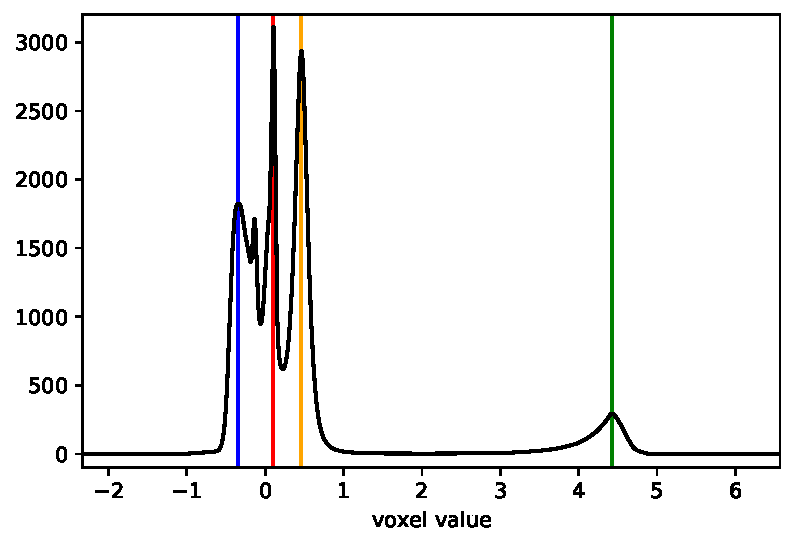
\includegraphics[width=\linewidth]{figures/1d_hist.pdf}
    \caption{1-dimensional histogram of the voxel values of a tomography. The blue line is air peak, the red line is the soft tissue peak, the green line is the bone peak, and the orange line is the implant peak.}
    \label{fig:1d-hist}
\end{figure}

\subsection{Preprocessing}\label{sec:preprocess}
To reduce the complexity of the segmentation process, we preprocess the data by removing redundant information.
From our work in another paper, we are able to obtain two masks: an \textit{implant mask} and a \textit{bone mask}.

Since the values of the implant material is radically different from the rest of the sample, obtaining the rough implant mask through global thresholding is trivial, as the orange line in~\Cref{fig:1d-hist} shows.
This mask is then refined, along with the internal gaps closed, giving us the implant mask. 
Using this mask, we are also able to remove the air making up half of the sample cylinder (depicted above the implant in the XY and to the left of the implant in the YZ cross sections of~\Cref{fig:3viewsample}), as the implant mask can show us the orientation of the implant. This squashes the blue peak from the histogram, leaving the two peaks marked by the red and green lines as being the most defined. 

As we are only interested in the voxels inside the bone, and that we know that the bone is the most prominent material left, we perform another coarse segmentation, by thresholding in between the two large distributions, choosing everything to the right of this threshold as the bone mask. These voxels are morphologically closed, to also consume the internal gaps of the bone region, which makes up the soft tissue inside the bone. The implant and bone region masks applied throughout the following steps to filter out noise in the tomography.

\subsection{Exploiting spatial information}
As described in~\Cref{sec:physics}, the voxel values vary according to their positioning, leading us to utilize spatial information in the tomography. 
%Show the correlation of x,y,z,r to histograms 2d
In order to include spatial information, we consider \textit{expanding} a dimension to produce multiple 1D histograms into a combined 2-dimensional histogram.
Each 2D histogram is computed by locking the dimension in question and produce the 1D histograms.
Specifically, we consider the radius ($r$) dimension from the center of the implant, as the voxel values vary the most closest to the implant. 
The algorithm for computing the 2-dimensional histogram for the radius can be seen in~\Cref{alg:2dhists} with the resulting 2D histogram plotted in~\Cref{fig:2dhists}.
From this plot, we see two prominent distributions that change along the $r$ axis.
However, this is not an accurate representation, as the edges of the implant is not uniformly spread across the longest axis of the implant, meaning that the radius does not represent the distance from the implant in high resolutions. This is shown in~\Cref{fig:edt-vs-diffusion}, where we see that a radius of constant value from the center has varying distance to the implant.

\carl{discuss the effects with references to the physics (previous section). Kunne jeg godt bruge hjælp til.}

% Kept for historical reasons.
%\begin{algorithm}
%    \caption{2-dimensional histograms. Allocation also implies zero initialization.}
%    \label{alg:2dhists}
%    \begin{algorithmic}
%        \Function {2D\_hist} {$voxels[n_z,n_y,n_x],c_x,c_y,n_{bins},v_{min},v_{max}$}
%            \State $n_r \gets \left\lfloor\sqrt{\left\lfloor \frac{n_x}{2} \right\rfloor^2 + \left\lfloor \frac{n_y}{2} \right\rfloor^2}\right\rfloor+1$
%            \State \textbf{allocate} $h_z[n_z,n_{bins}], h_y[n_y,n_{bins}]$
%            \State \textbf{allocate} $h_x[n_x,n_{bins}], h_r[n_r,n_{bins}]$
%            \For {$z,y,x$ \textbf{in} $0{:}n_z,0{:}n_y,0{:}n_x$}
%                \State $v \gets voxels[z,y,x]$
%                \If {$v_{min} \leq v \leq v_{max}$}
%                    \State $v_{i} \gets (n_{bins}-1) \cdot \frac{v - v_{min}}{v_{max} - v_{min}}$
%                    \State $r \gets \left\lfloor\sqrt{(x-c_x)^2 + (y-c_y)^2}\right\rfloor$
%                    \State $h_z[z,v_{i}]{+}{+}$
%                    \State $h_y[y,v_{i}]{+}{+}$
%                    \State $h_x[x,v_{i}]{+}{+}$
%                    \State $h_r[r,v_{i}]{+}{+}$
%                \EndIf
%            \EndFor
%            \Return $h_z,h_y,h_z,h_r$
%        \EndFunction
%    \end{algorithmic}
%\end{algorithm}

\begin{algorithm}
    \caption{2-dimensional radius histogram.}
    \label{alg:2dhists}
    \begin{algorithmic}
        \Function {hist\_r} {$voxels[n_z,n_y,n_x],c_x,c_y,n_{bins},v_{min},v_{max}$}
            \For {$z,y,x$ \textbf{in} $0{:}n_z,0{:}n_y,0{:}n_x$}
                \State $v \gets voxels[z,y,x]$
                \If {$v_{min} \leq v \leq v_{max}$}
                    \State $v_{i} \gets (n_{bins}-1) \cdot \frac{v - v_{min}}{v_{max} - v_{min}}$
                    \State $r \gets \left\lfloor\sqrt{(x-c_x)^2 + (y-c_y)^2}\right\rfloor$
                    \State $h_r[r,v_{i}]{+}{+}$
                \EndIf
            \EndFor
            \Return $h_r$
        \EndFunction
    \end{algorithmic}
\end{algorithm}

\begin{figure}
    \centering
    %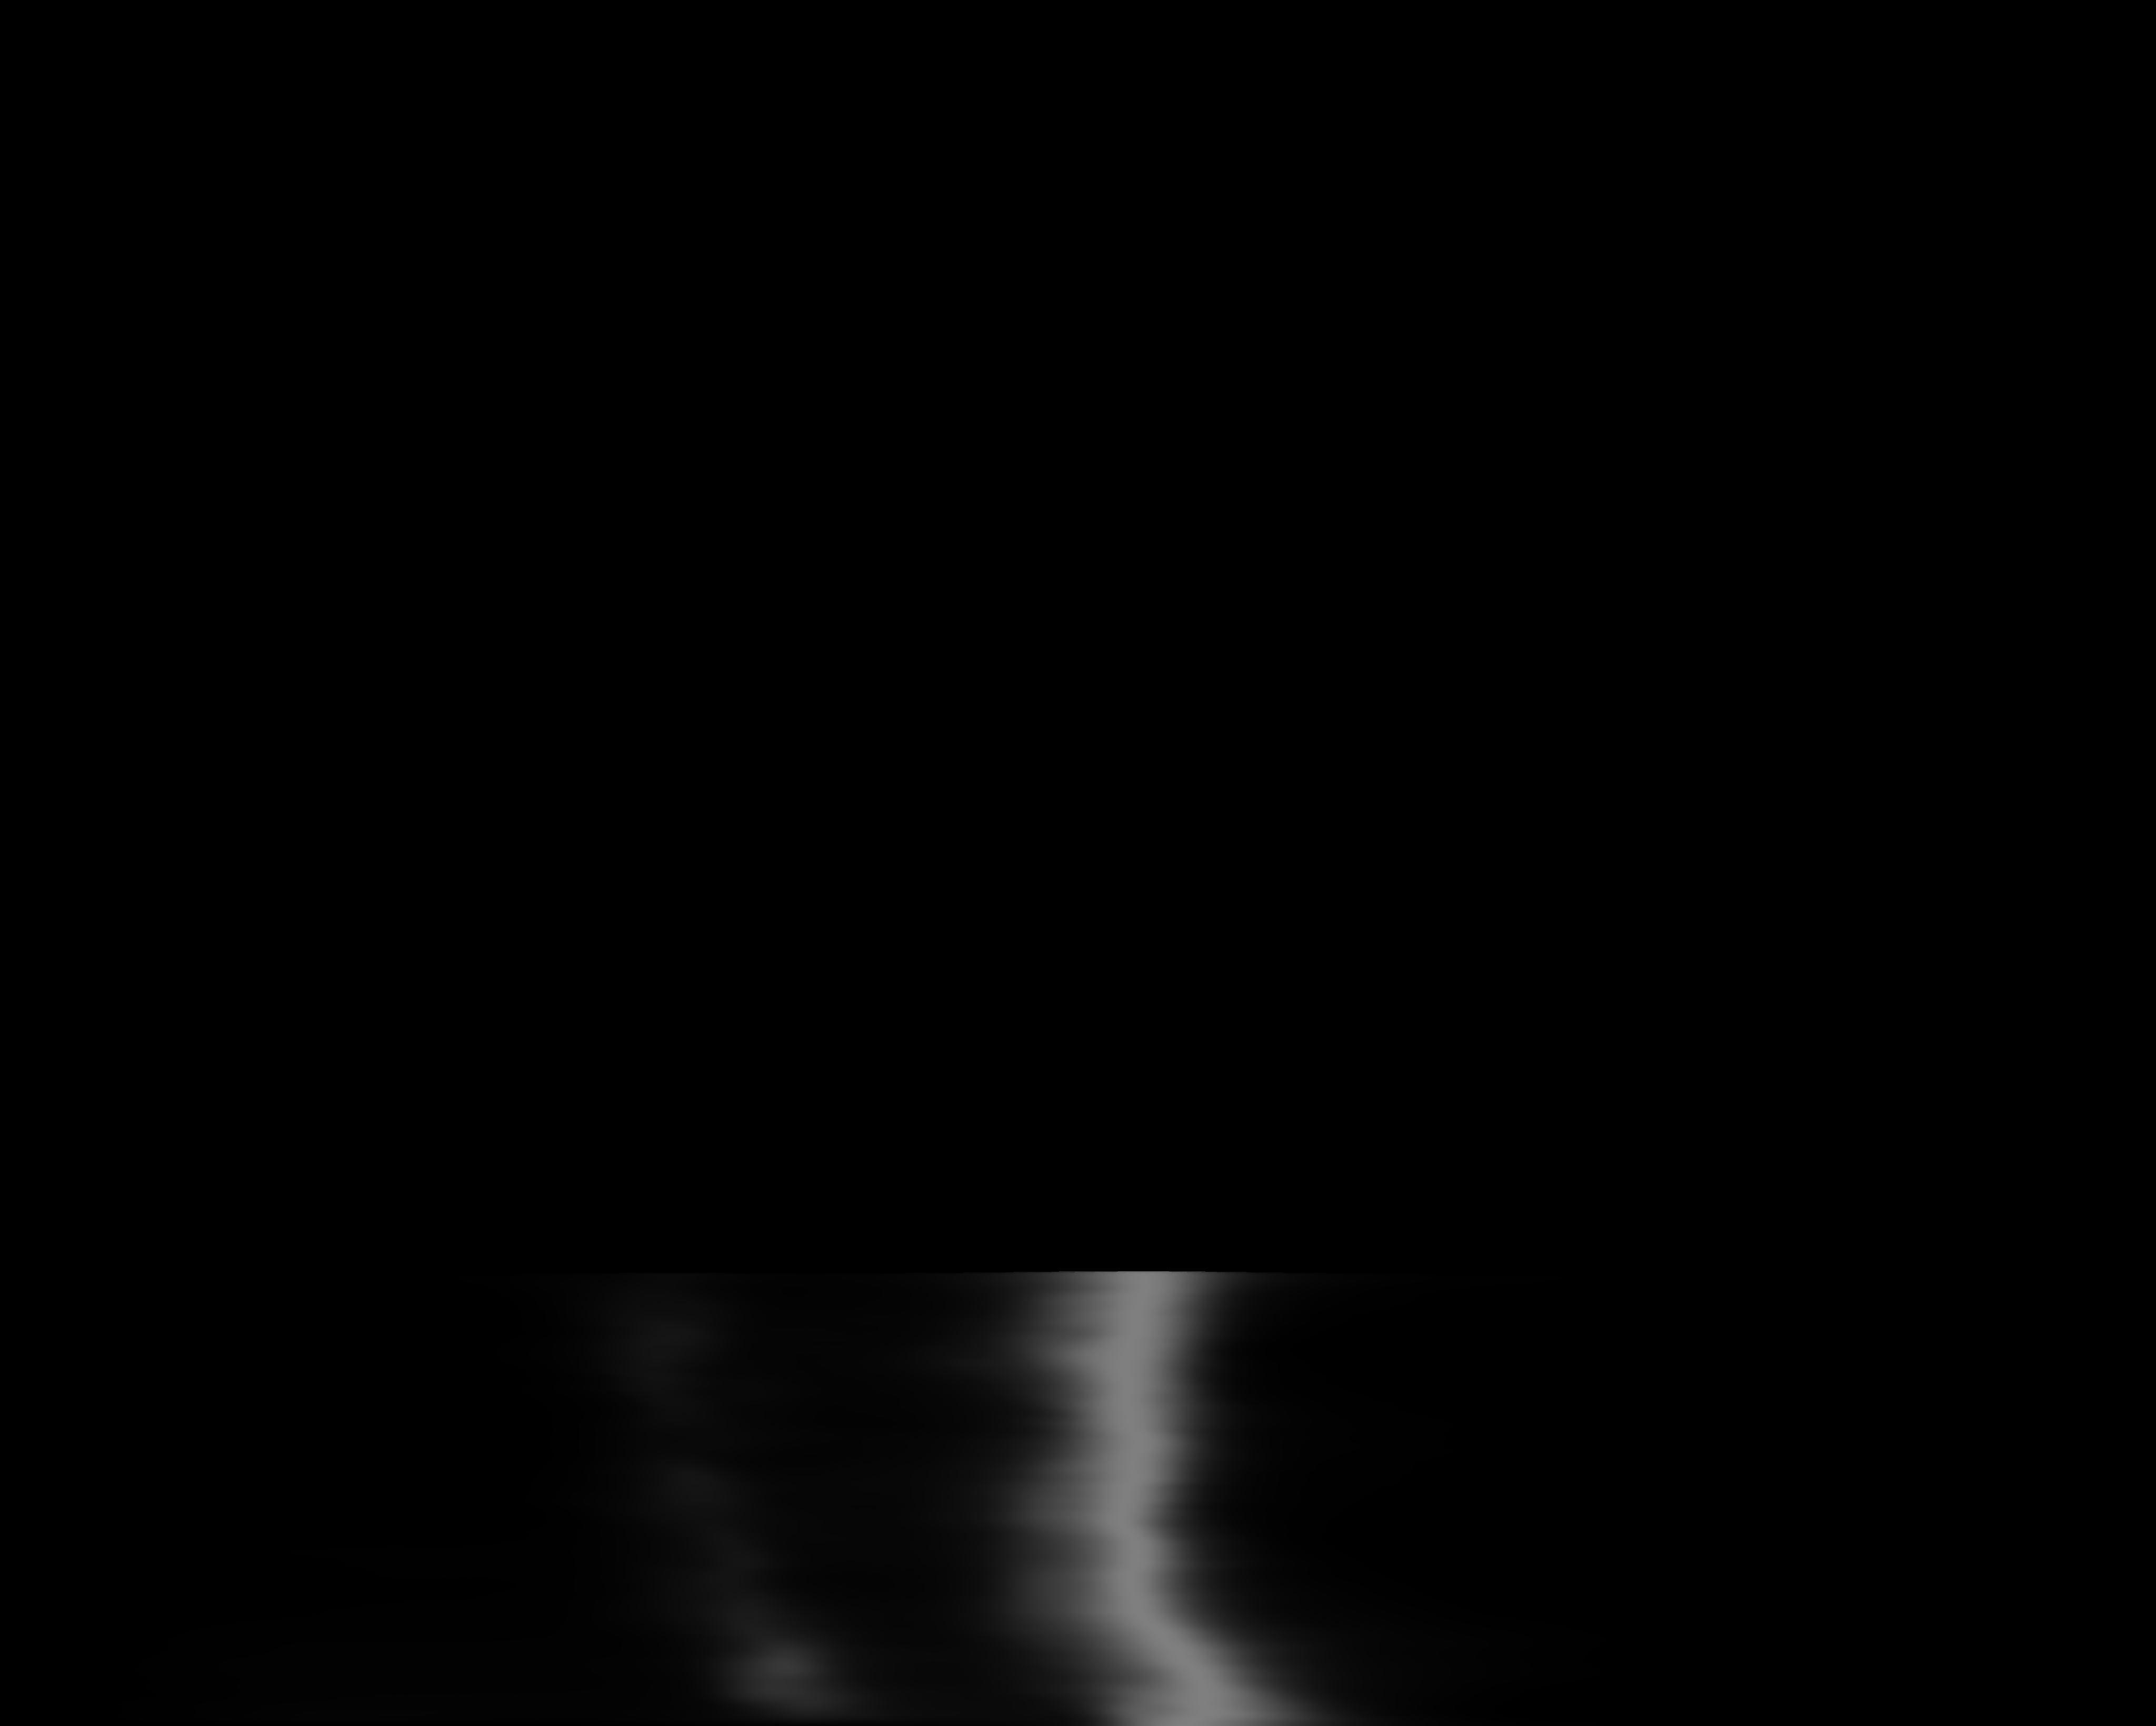
\includegraphics[width=.49\linewidth]{figures/zb-bone_region3.png}
    %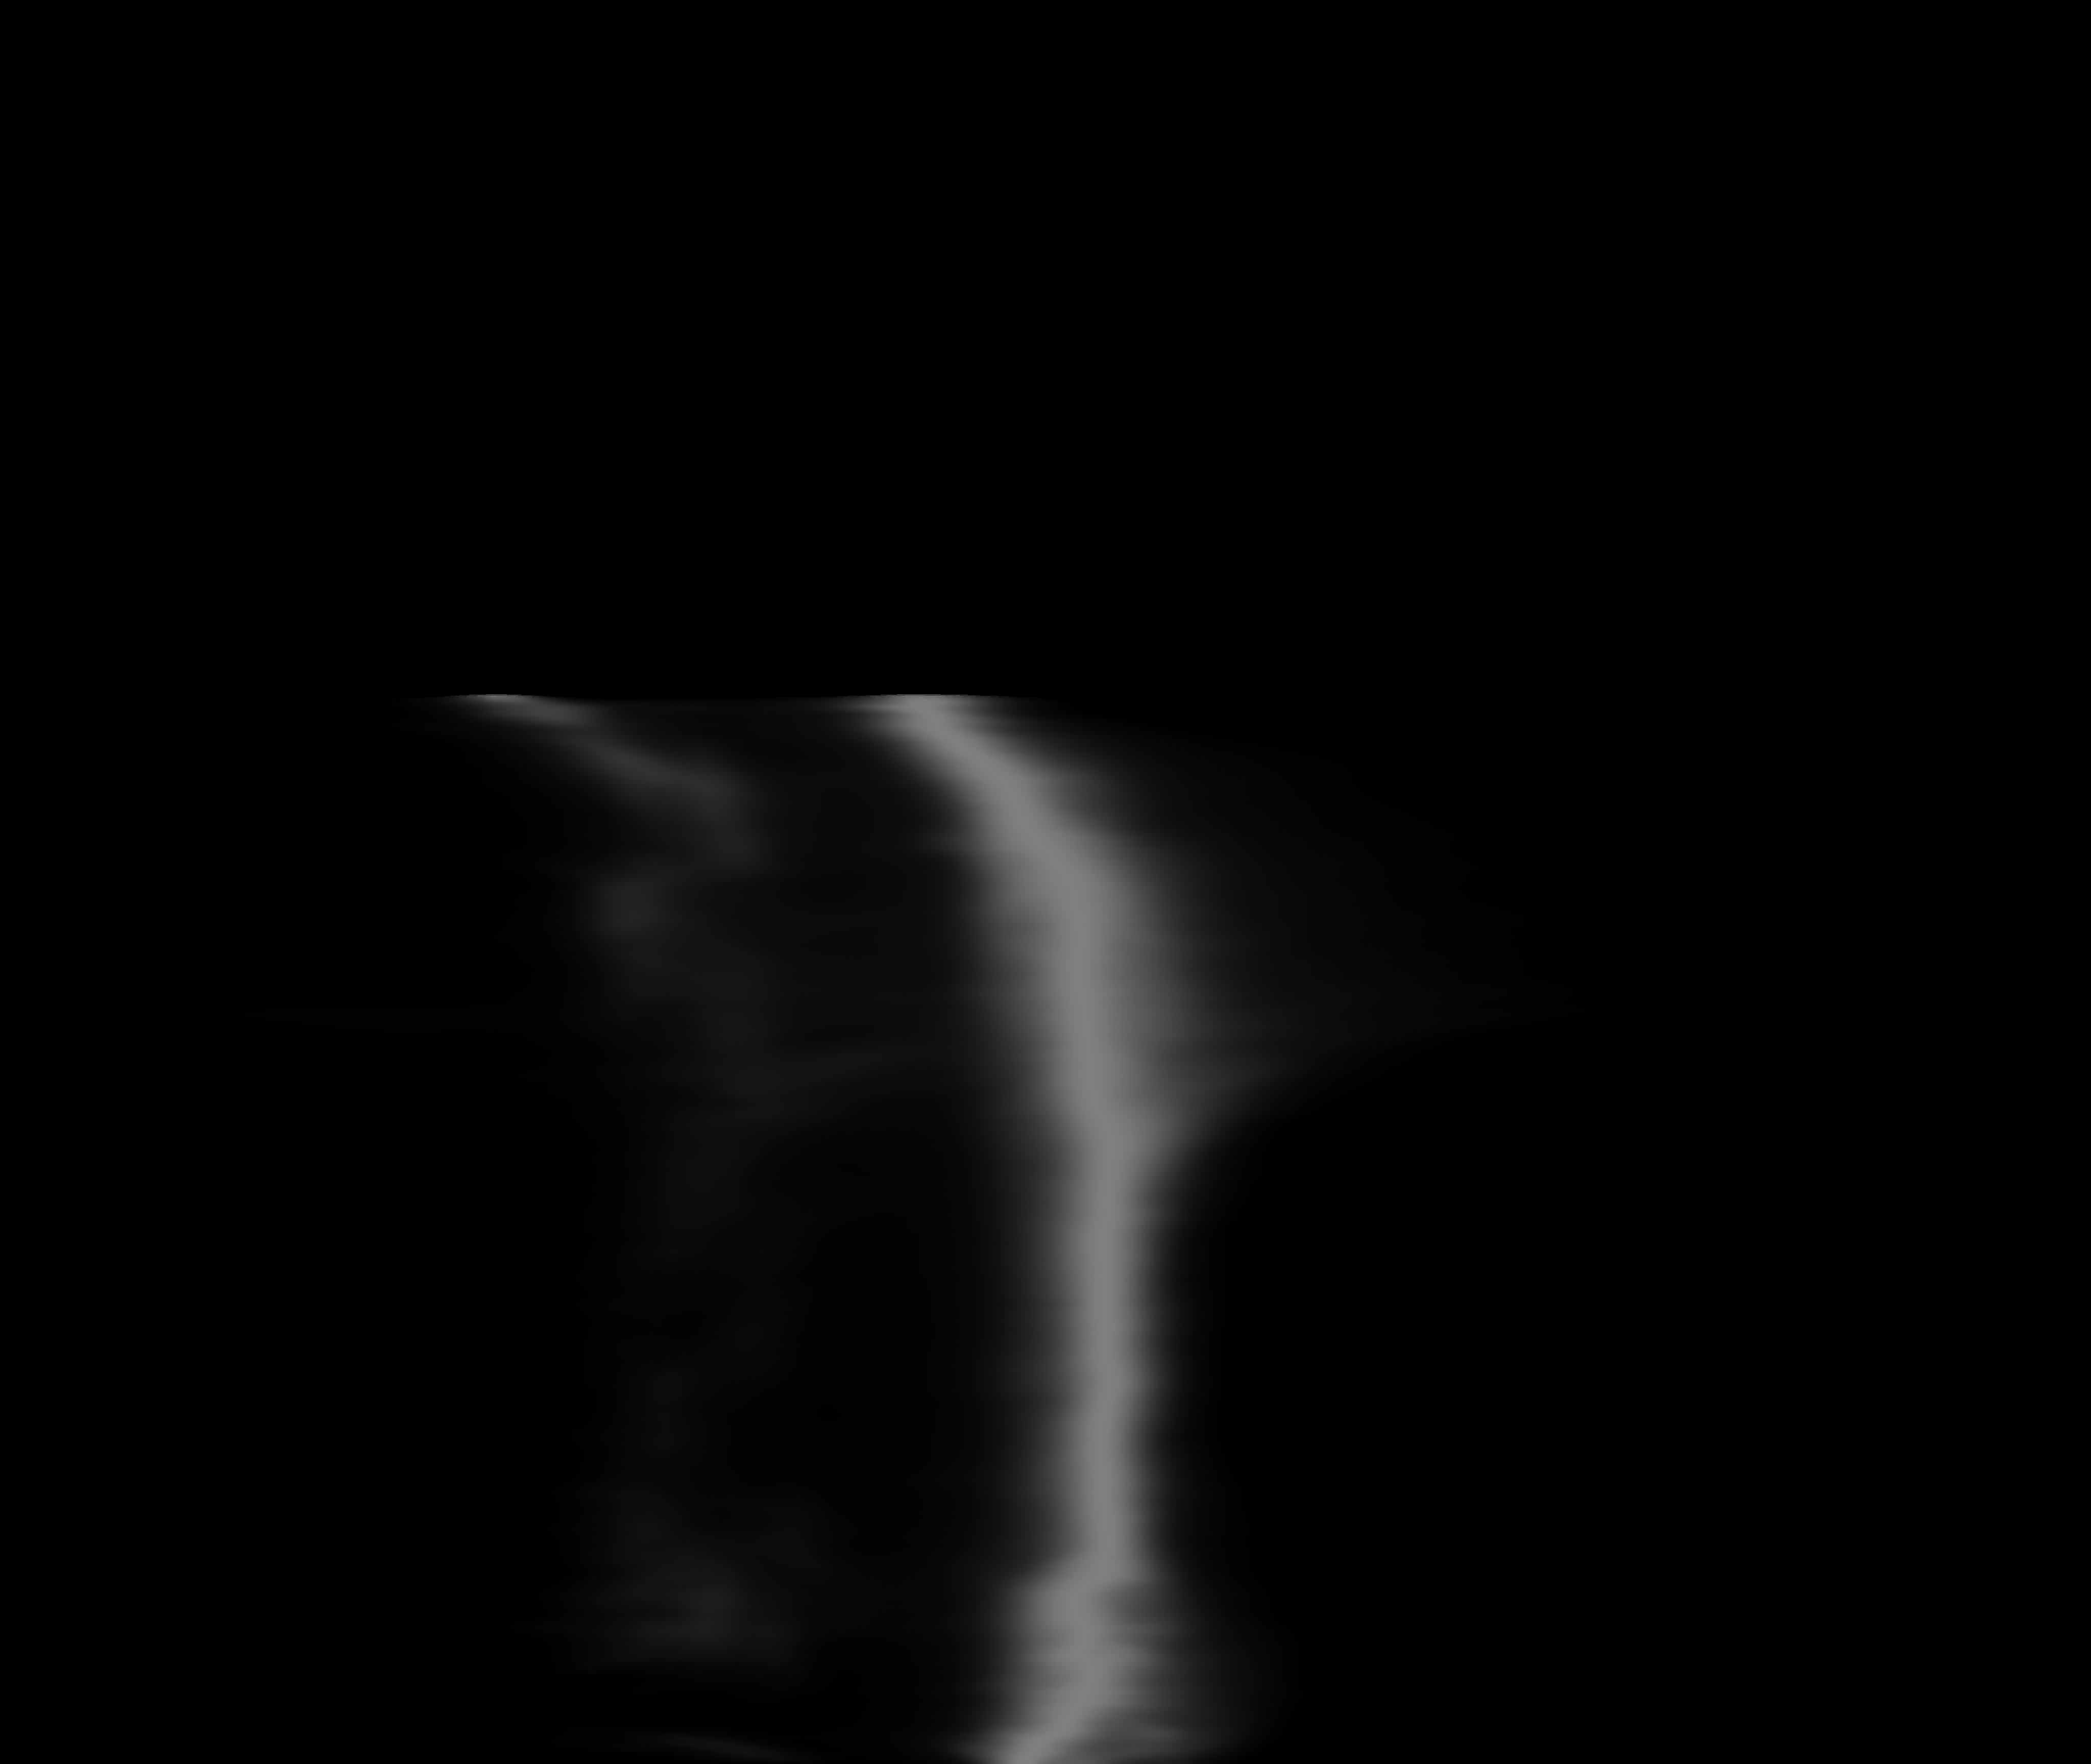
\includegraphics[width=.49\linewidth]{figures/yb-bone_region3.png}
    %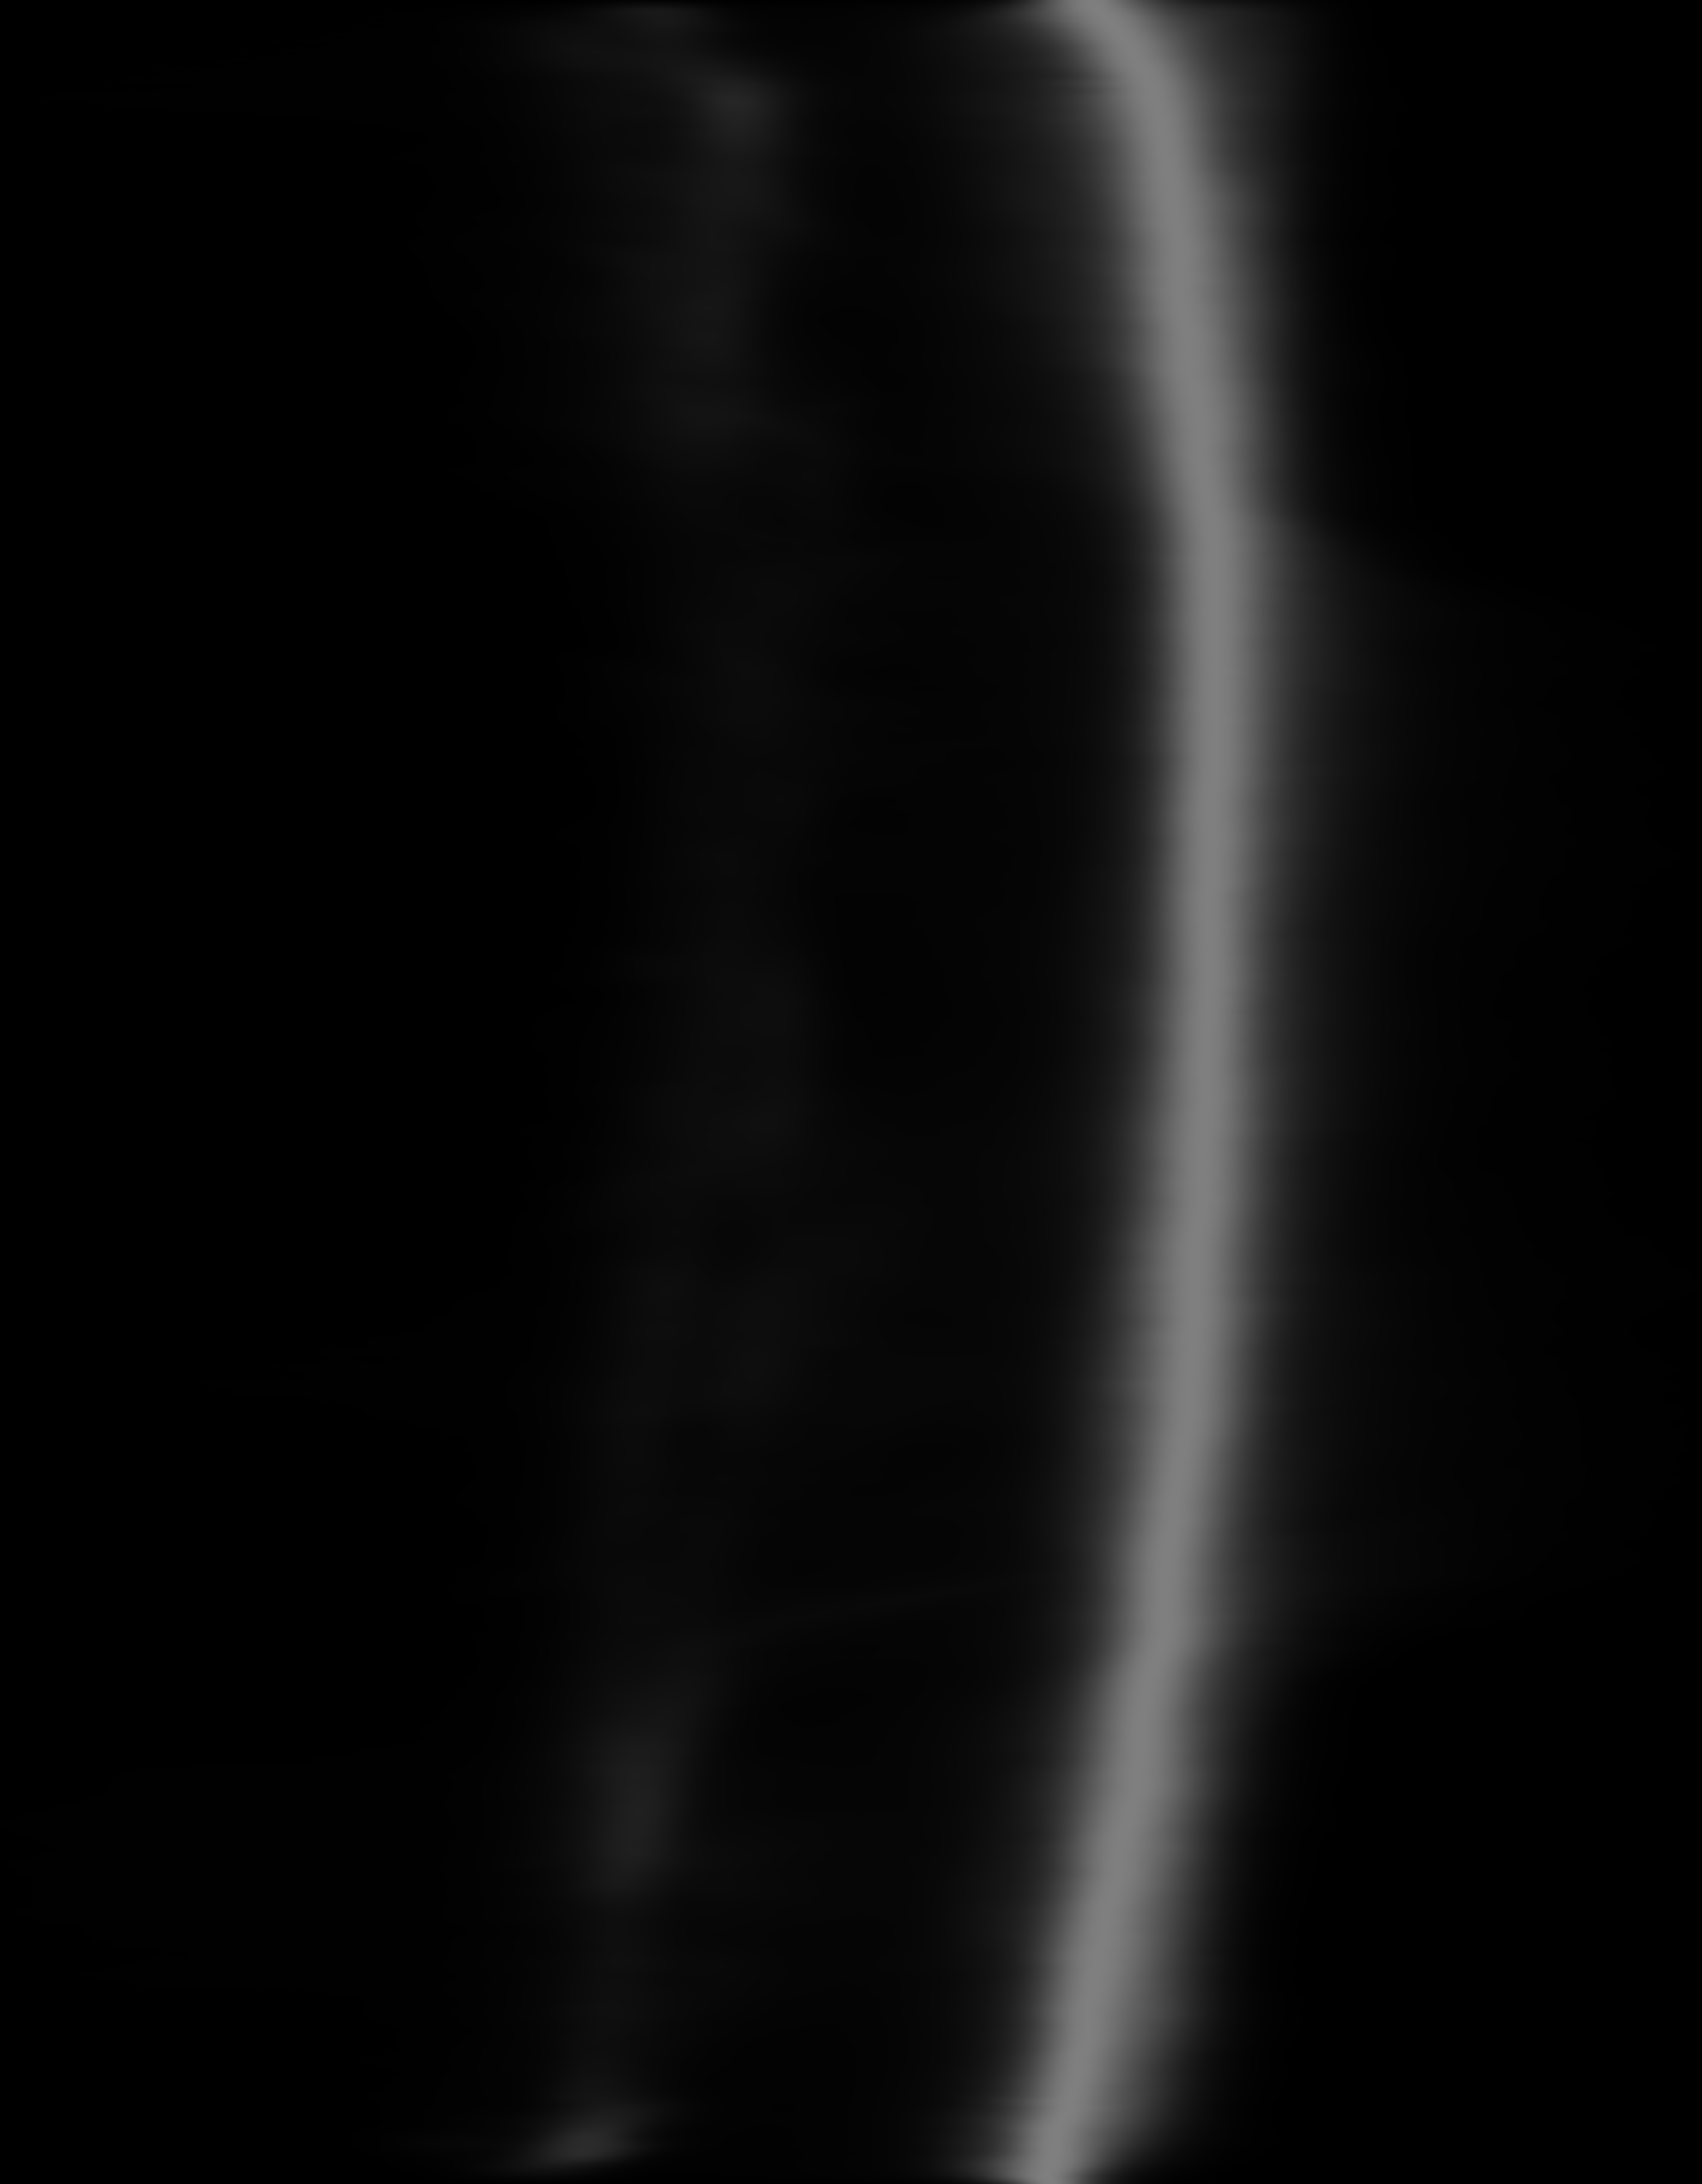
\includegraphics[width=.49\linewidth]{figures/xb-bone_region3.png}
    %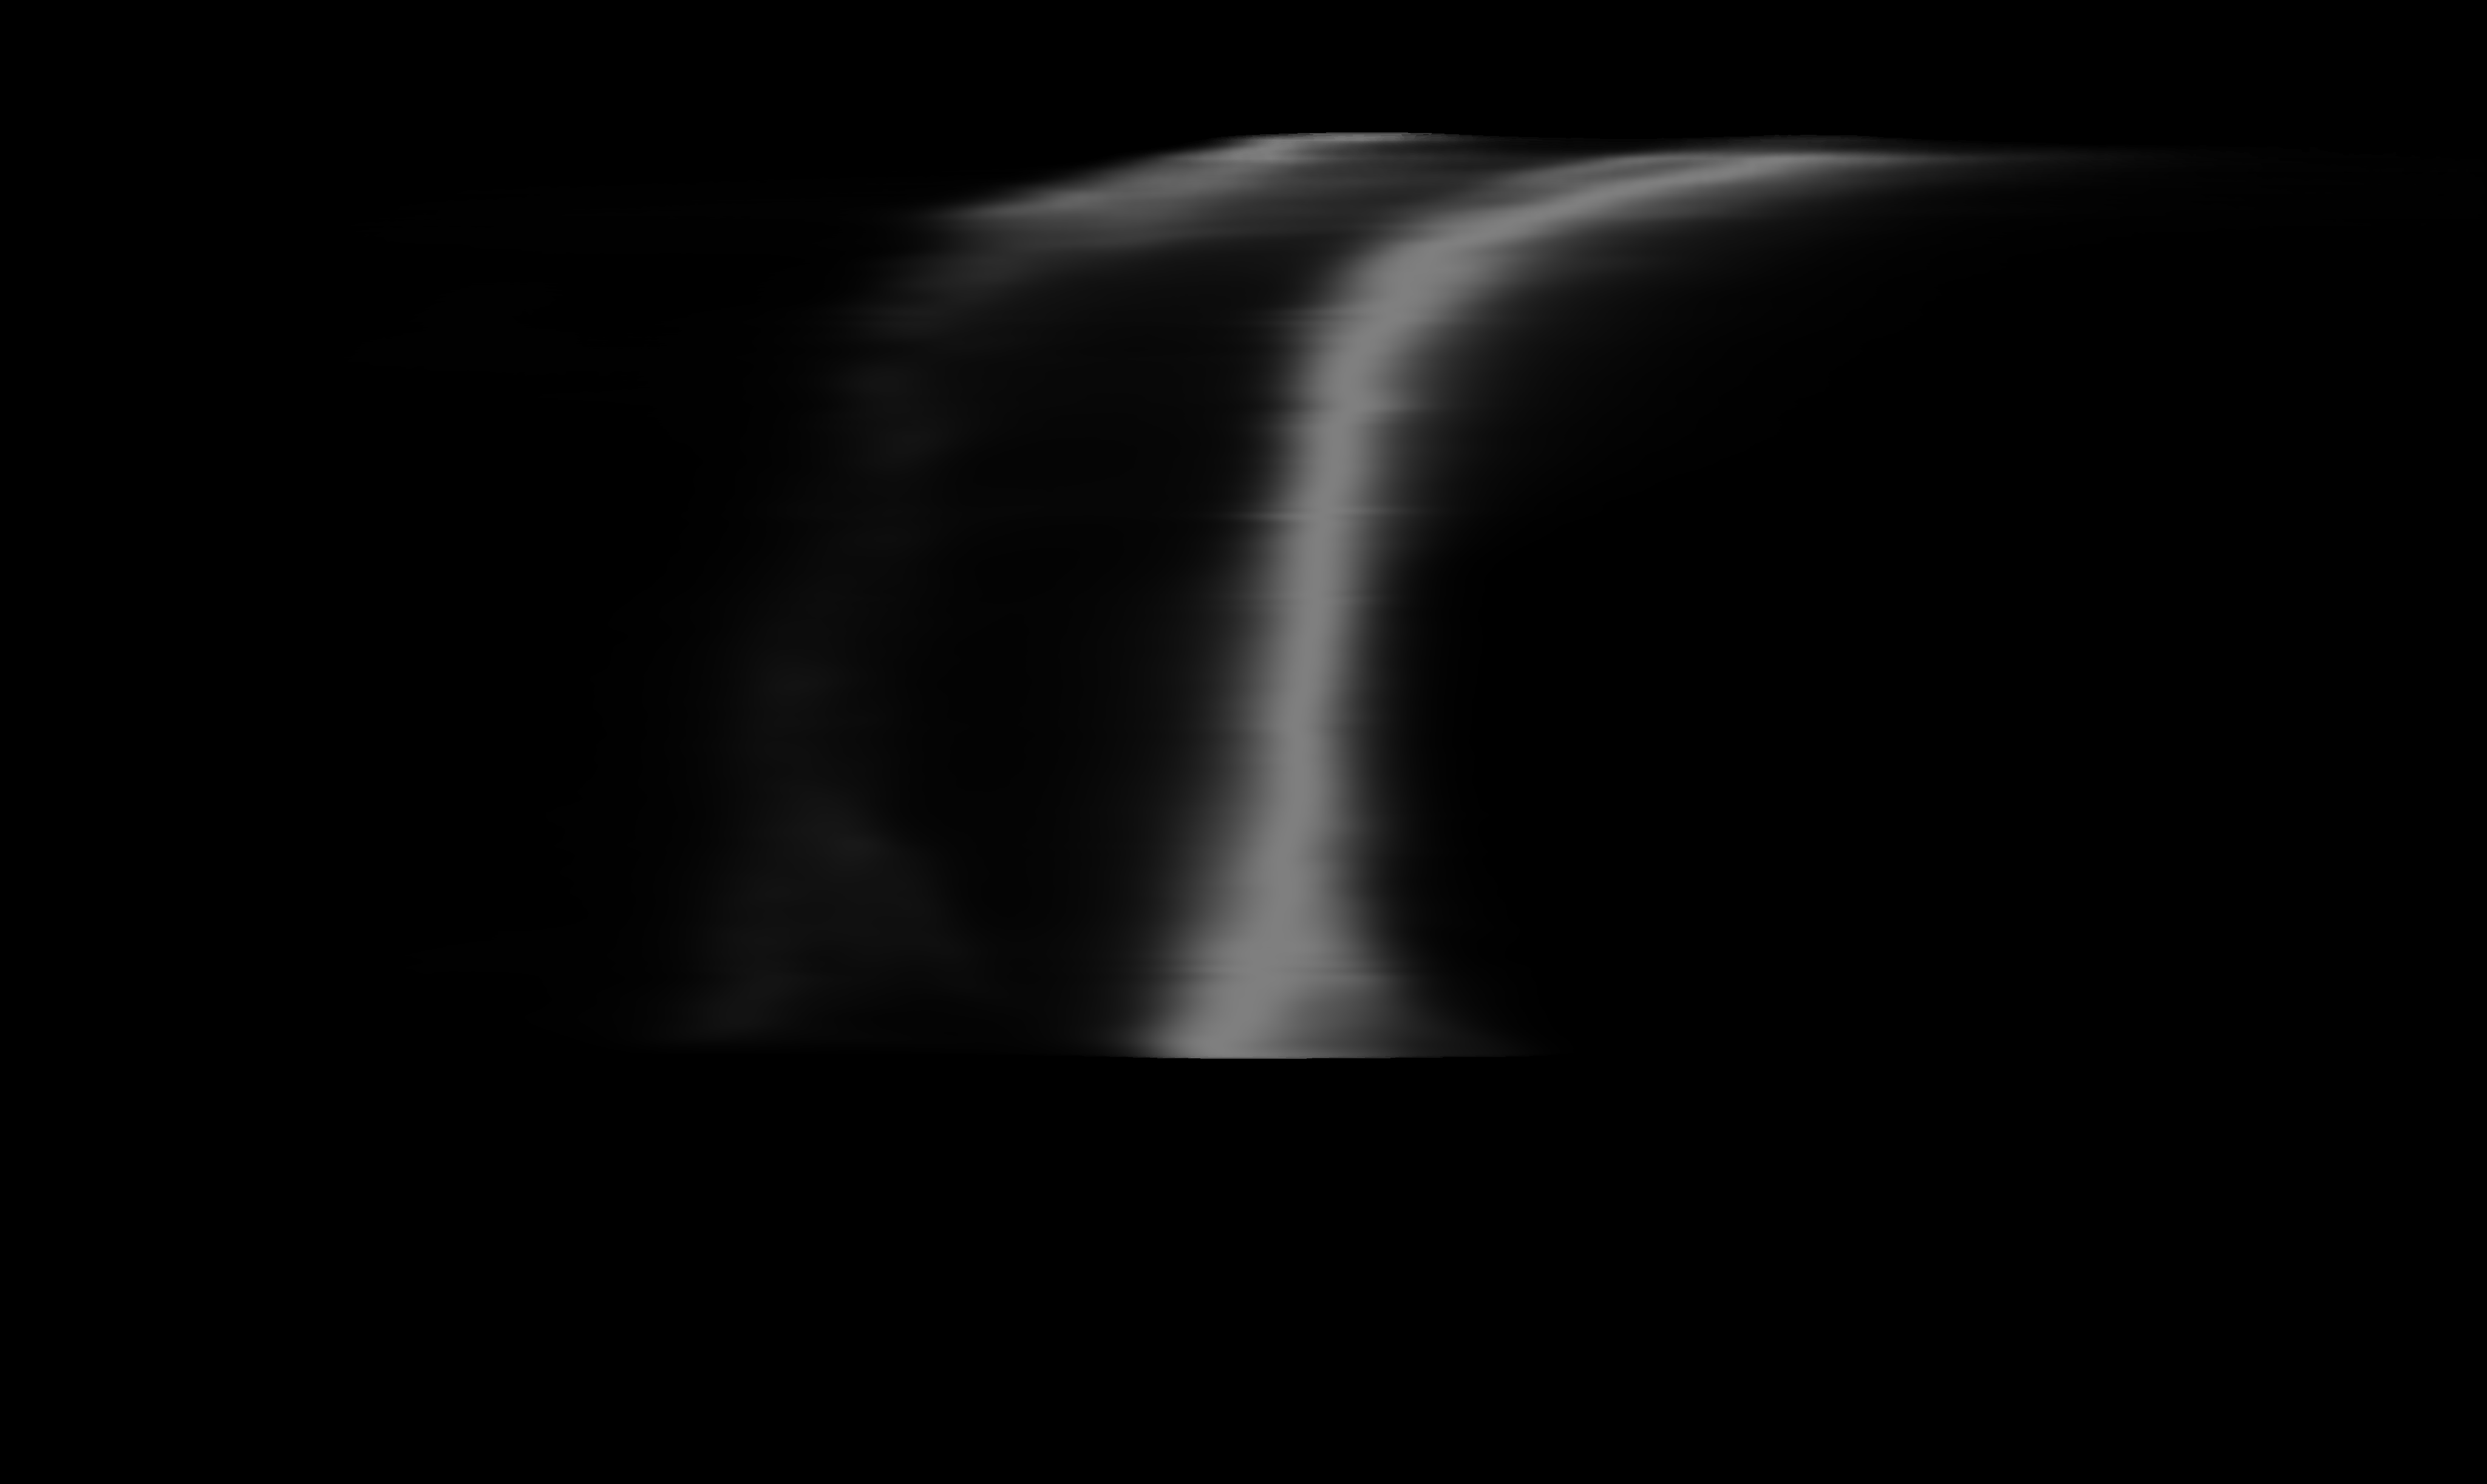
\includegraphics[width=\linewidth]{figures/rb-bone_region3.png}
    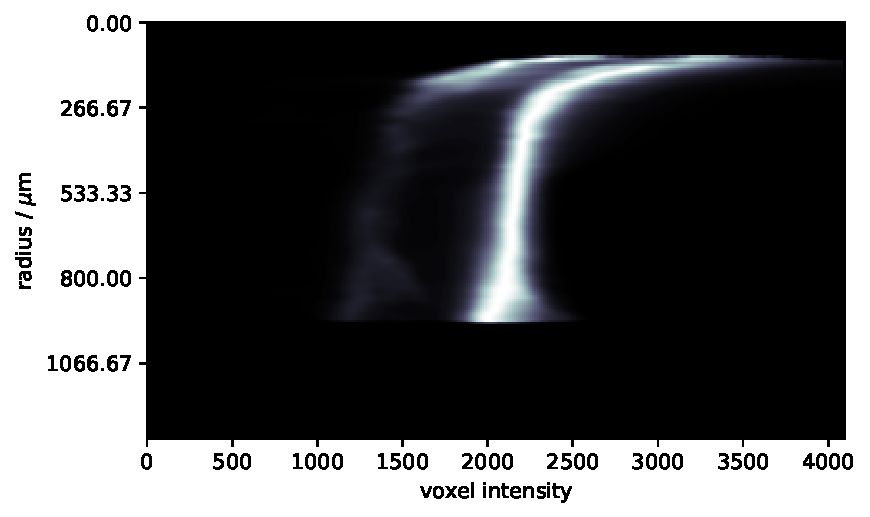
\includegraphics[width=\linewidth]{figures/rb-bone_region3.pdf}
    \caption{2D radius histogram. The y-axis depicts radius, with the x-axis being voxel value.}
    \label{fig:2dhists}
\end{figure}

\subsection{Field histograms}
%Show that the fields can perfectly seperate
%discuss all the way to implant contact
In order to obtain spatial information based on the relation to the implant, we construct two \textit{field} representations: Euclidian Distance Transform (EDT) and Diffusion.

%EDT is good overall, but difficult close to the implant.
EDT computes each voxel as the euclidian distance to the implant. 
This makes for a generally good representation for all but the voxels that are close to the implant.
The shortcoming near the implant is mainly due to the fact that the voxels in the grooves of the implant has the same distance, and thus gets the same value, as the voxels next to the threads of the implant, as is shown in~\Cref{fig:edt-vs-diffusion}.
As discussed in~\Cref{sec:beam-hardening}, the implant produces a "glowing" effect, which should be corrected by having higher field values for voxels surrounded by implant.

%Use diffusion to "zoom in" on the implant, as it is good close to the implant, but throws everything far away into the same bin
To get better correction close to the implant, we utilize diffusion where the implant "glows" further accumulating the value when a voxel is surrounded by implant.
This is shown in~\Cref{fig:edt-vs-diffusion}, where the voxels in the grooves are affected by multiple implant voxels.
A slice of the resulting diffusion field can be seen in~\Cref{fig:field-slice}.

\begin{figure}
    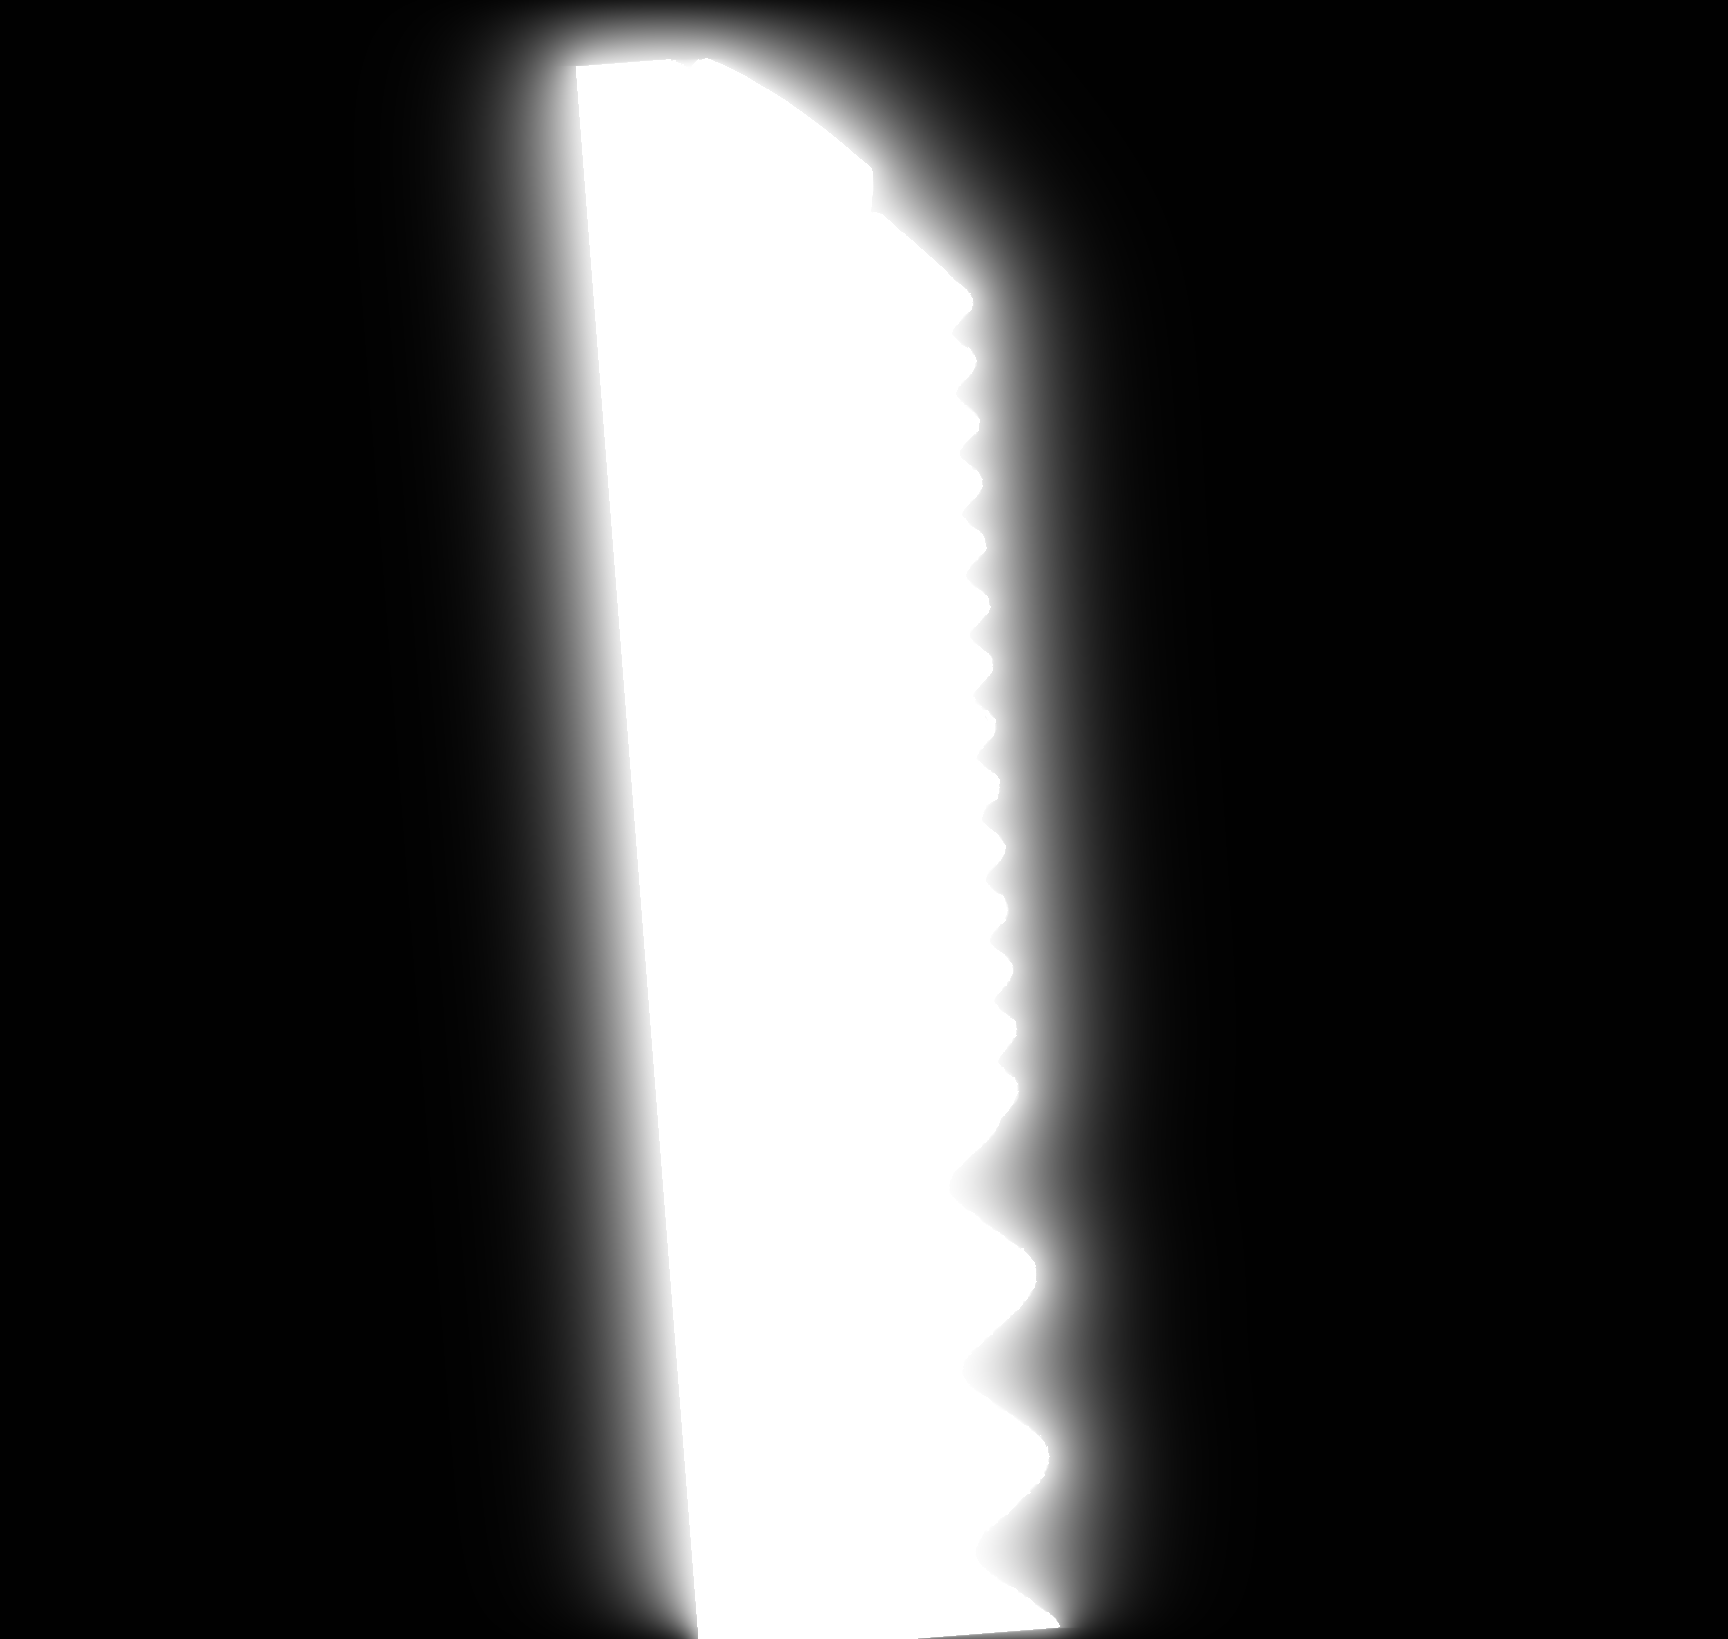
\includegraphics[width=\linewidth]{figures/770c_pag-gauss-yz.png}
    \caption{A slice of the diffusion field in the YZ plane.}
    \label{fig:field-slice}
\end{figure}

\begin{figure}
    \vspace{-1.5cm}
    \centering
    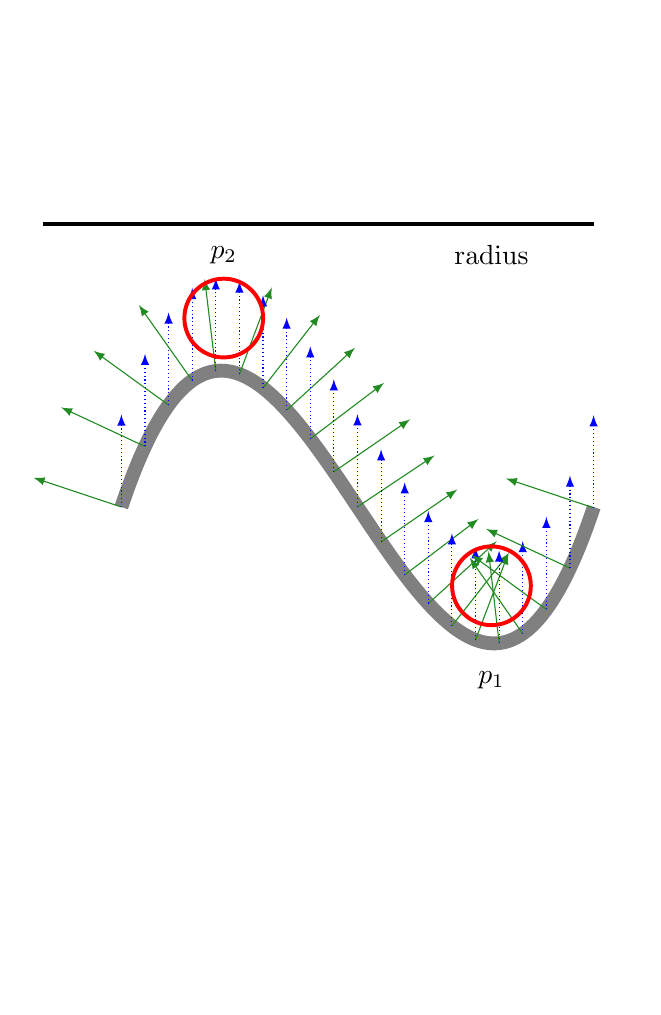
\begin{tikzpicture}[scale=2.0]
        \draw[gray,line width=5pt] (0,0)
        .. controls (1,3) and (2,-3) .. (3,0)
        \foreach \p in {0,5,...,100} {
          node[sloped,inner sep=0cm,above,pos=\p*0.01,
          anchor=south,
          minimum height=1.0cm,minimum width=1.0cm]
          (N \p){}
        }
        \foreach \p in {0,5,...,100} {
          node[midway,above,inner sep=0cm,above,pos=\p*0.01,
          anchor=south,
          minimum height=1.0cm,minimum width=1.0cm]
          (N2 \p){}
        }
        ;
        \foreach \p in {0,5,...,100} {
          \draw[-latex,ForestGreen] (N \p.south) -- (N \p.north);
          \draw[-latex,blue,densely dotted] (N2 \p.south) -- (N2 \p.north);
        }
        \draw[red, line width=0.5mm] (0.65,1.20) circle (0.25cm);
        \node at (0.65,1.60) {$p_2$};
        \draw[red, line width=0.5mm] (2.35,-0.5) circle (0.25cm);
        \node at (2.35,-1.10) {$p_1$};
        \draw[black, line width=0.5mm] (-0.5,1.8) -- (3.0,1.8);
        \node at (2.35,1.60) {radius};
      \end{tikzpicture}
      \vspace{-3.5cm}
    \caption{Visualization of the different field computations close to the implant in the YZ plane. The EDT is depicted in green, where we see that $p_1$ and $p_2$ has the same distance. Diffusion is depicted in blue, where we see multiple arrows contributing to the value of $p_1$.}
    \label{fig:edt-vs-diffusion}
\end{figure}

While Diffusion works well on voxels close to the implant, it assigns the same value to the voxels far from the implant. 
As such, an optimal solution is to use both the EDT and the diffusion field to better represent both voxels that are far away, as well as the ones that are close to the implant.
We achieve this by adding the two fields together, producing a final combined field.

%Show that the distance to the implant in edt will be the same in the grooves of the screw compared to the threads of the screw. This is "fixed" with diffusion, as the grooves will be brigher as it is surrounded by more implant.

\subsection{Walkthrough of the method}
This section will describe the steps of the method in detail for going from tomography to material probability distributions.
\carl{flavortext}

\subsubsection{Overview}
%Coarse steps, explain the idea
The coarse steps of the segmentation method are:
\begin{enumerate}
    \item Compute the EDT and Diffusion fields to give each voxel spatial information about its relation to the implant.
    \item Compute frequency distributions of voxel values as functions of field values as 2D histograms.
    \item Find the materials within the 2D histograms as ridges, using image processing techniques.
    \item From the ridges, compute initial approximate frequence distributions of each material, which are then optimized to fit the 2D histograms. 
    \item From the optimized distributions, we derive probability distributions for material classification.
\end{enumerate}
The computed distributions approximate the conditional probabilities $P(m|v,x)$ that a particular voxel
is material $m$ given that it has value $v$ and field value $x$. 

\james{TODO: Forklar bedre. Adskil ny segmenteringsmetode og anvendelse til BIC}

These steps are also summarized in the flow chart in~\Cref{fig:flowchart}.

\begin{figure}
    \centering
    \begin{tikzpicture}
        %\node (voxels) at (0,2) {tomography};
        %\node[anchor=east] (implant) at (-1,1) {implant mask};
        %\node[anchor=west] (bone) at (1,1) {bone mask};
        %\draw[draw] (implant.north west) rectangle (bone.south east);

        \node[draw] (field) at (0,0) {1. Compute fields};
        \node[draw, below = of field] (hists) {2. Compute 2D histograms};
        \node[draw, below = of hists] (curvs) {3. Find Ridges};
        \node[draw, below = of curvs] (probs) {4. Compute probabilities};
        \node[draw, below = of probs] (segm)  {5. Segment the voxels};
        \node[draw, below = of segm]  (blood) {6. Compute blood network};
        \node[draw, below = of blood] (bic)   {7. Compute bone- and blood-implant contact};

        %\path[draw, ->] (voxels) -- (field);
        %\path[draw, ->] (implant) -| ([shift={(-.5,0)}]field.north);
        %\path[draw, ->] (bone) -| ([shift={(.5,0)}]field.north);
        \path[draw, ->] (field) -- (hists);
        \path[draw, ->] (hists) -- (curvs);
        \path[draw, ->] (curvs) -- (probs);
        \path[draw, ->] (probs) -- (segm);
        \path[draw, ->] (segm) -- (blood);        
        \path[draw, ->] (blood) -- (bic);
    \end{tikzpicture}
    \caption{Flowchart depicting the steps of the method.
    \carl{Kan måske arrangeres ligesom Davids ting oversigt? Giver måske kun mening hvis der var mere end bare segmentation -> bic}}
    \label{fig:flowchart}
\end{figure}

\subsubsection{Segmentation}
The segmentation is computed in steps 1-5. For each step we will describe the process, showing the algorithm where applicable, along with the the intermediate results. 

\vspace{\baselineskip}
\noindent\textit{\textbf{1. Field computations}}
Both fields are computed from the implant mask, as described in~\Cref{sec:preprocess}.
EDT is computed using the Python package \texttt{edt}~\cite{pypi-edt}. It takes the implant mask and sets every non-set voxel to be the euclidian distance to the nearest implant voxel.

For diffusion, rather than solving the diffusion equation, we approximate using multiple convolutions of a 3D-gaussian kernel.
Furthermore, instead of a single pass with a 3D-kernel, we apply 3 1D convolutions, one in each dimension, to the tomography, obtaining the same result as a regular 3D-gaussian kernel.
The algorithm can be seen in~\Cref{alg:diffusion}, an XZ slice in~\Cref{fig:field-slice}.

\begin{algorithm}
    \caption{Diffusion approximation.}
    \label{alg:diffusion}
    \begin{algorithmic}
        \Function {Diffusion} {$voxels[n_z*n_y*n_x], repitions, kernel[2*k+1]$}
            \State $S \gets [n_y * n_x, n_x, 1]$
            \State $N \gets [n_z, n_y, n_x]$
            \State $buf_0[:] \gets voxels[:]$
            \For {$rep$ \textbf{in} $repitions$}
                \For {$dim$ \textbf{in} $dimensions$}
                    \For {$z,y,x$ \textbf{in} $0{:}n_z,0{:}n_y,0{:}n_x$}
                        \State $X \gets [z,y,x]$
                        \State $i_{start} \gets - \min (k, X[dim])$
                        \State $i_{end} \gets \min (k, N[dim] - X[dim] - 1)$
                        \State $i_{global} \gets z*S[0] + y*S[1] + x*S[2]$
                        \For {$i$ \textbf{in} $i_{start}:i_{end}$}
                            \State $i_{offset} \gets i_{global} + i*S[dim]$
                            \State $buf_1[index] \gets buf_0[i_{offset}] * kernel[i+k]$
                        \EndFor
                    \EndFor
                    \State $buf_0[:] \gets buf_1[:]$
                \EndFor
            \EndFor
            \Return $buf_0$
        \EndFunction
    \end{algorithmic}
\end{algorithm}

%EDT + Diffusion
To obtain good seperation both close to the implant and far away, we combine the two fields into a single one as shown in~\Cref{alg:field-comb}.

\begin{algorithm}
    \caption{Field combination}
    \label{alg:field-comb}
    \begin{algorithmic}
        \Function {field\_combine} {$f_{edt}, f_{dif}$}
            \State $r \gets f_{dif} - \frac{f_{edt}}{\max (f_{edt})}$
            \State $r \gets r - \min (f_{dif})$
            \State $r \gets \frac{r}{\max (f_{dif})}$

            \Return $r$
        \EndFunction
    \end{algorithmic}
\end{algorithm}

\vspace{\baselineskip}
\noindent\textbf{2. 2D histograms} \\

From the combined fields we compute a 2D histogram with the field value on the y-axis and the voxel value on the x-axis. 
This allows us to see the distribution of voxel values, based off their relative position from the implant.
The algorithm for the field histogram can be seen in~\Cref{alg:field-hist} with a plot of the resulting histogram in~\Cref{fig:field-hist}.
We see that the voxel values shift based off how close to the implant clearly showing two seperable distributions.

\begin{algorithm}
    \caption{Field 2D histograms.}
    \label{alg:field-hist}
    \begin{algorithmic}
        \Function {Field\_hist} {$voxels[n_z,n_y,n_x], field[n_z,n_y,n_x],$ \newline $v_{bins}, v_{min}, v_{max}, f_{bins}, f_{min}, f_{max}$}
            \For {$z,y,x$ \textbf{in} $0{:}n_z,0{:}n_y,0{:}n_x$}
                \State $v \gets voxels[z,y,x]$
                \If {$v_{min} \leq v \leq v_{max}$}
                    \State $f \gets voxels[z,y,x]$
                    \If {$f_{min} \leq f \leq f_{max}$}
                        \State $v_i \gets (v_{bins} - 1) - \frac{v - v_{min}}{v_{max} - v_{min}}$
                        \State $f_i \gets (f_{bins} - 1) - \frac{f - f_{min}}{f_{max} - f_{min}}$
                        \State $h[f_i,v_i]{+}{+}$
                    \EndIf
                \EndIf
            \EndFor
            \Return $h$
        \EndFunction
    \end{algorithmic}
\end{algorithm}
\carl{look at indenting the function arguments in~\Cref{alg:field-hist}}

\begin{figure}
    %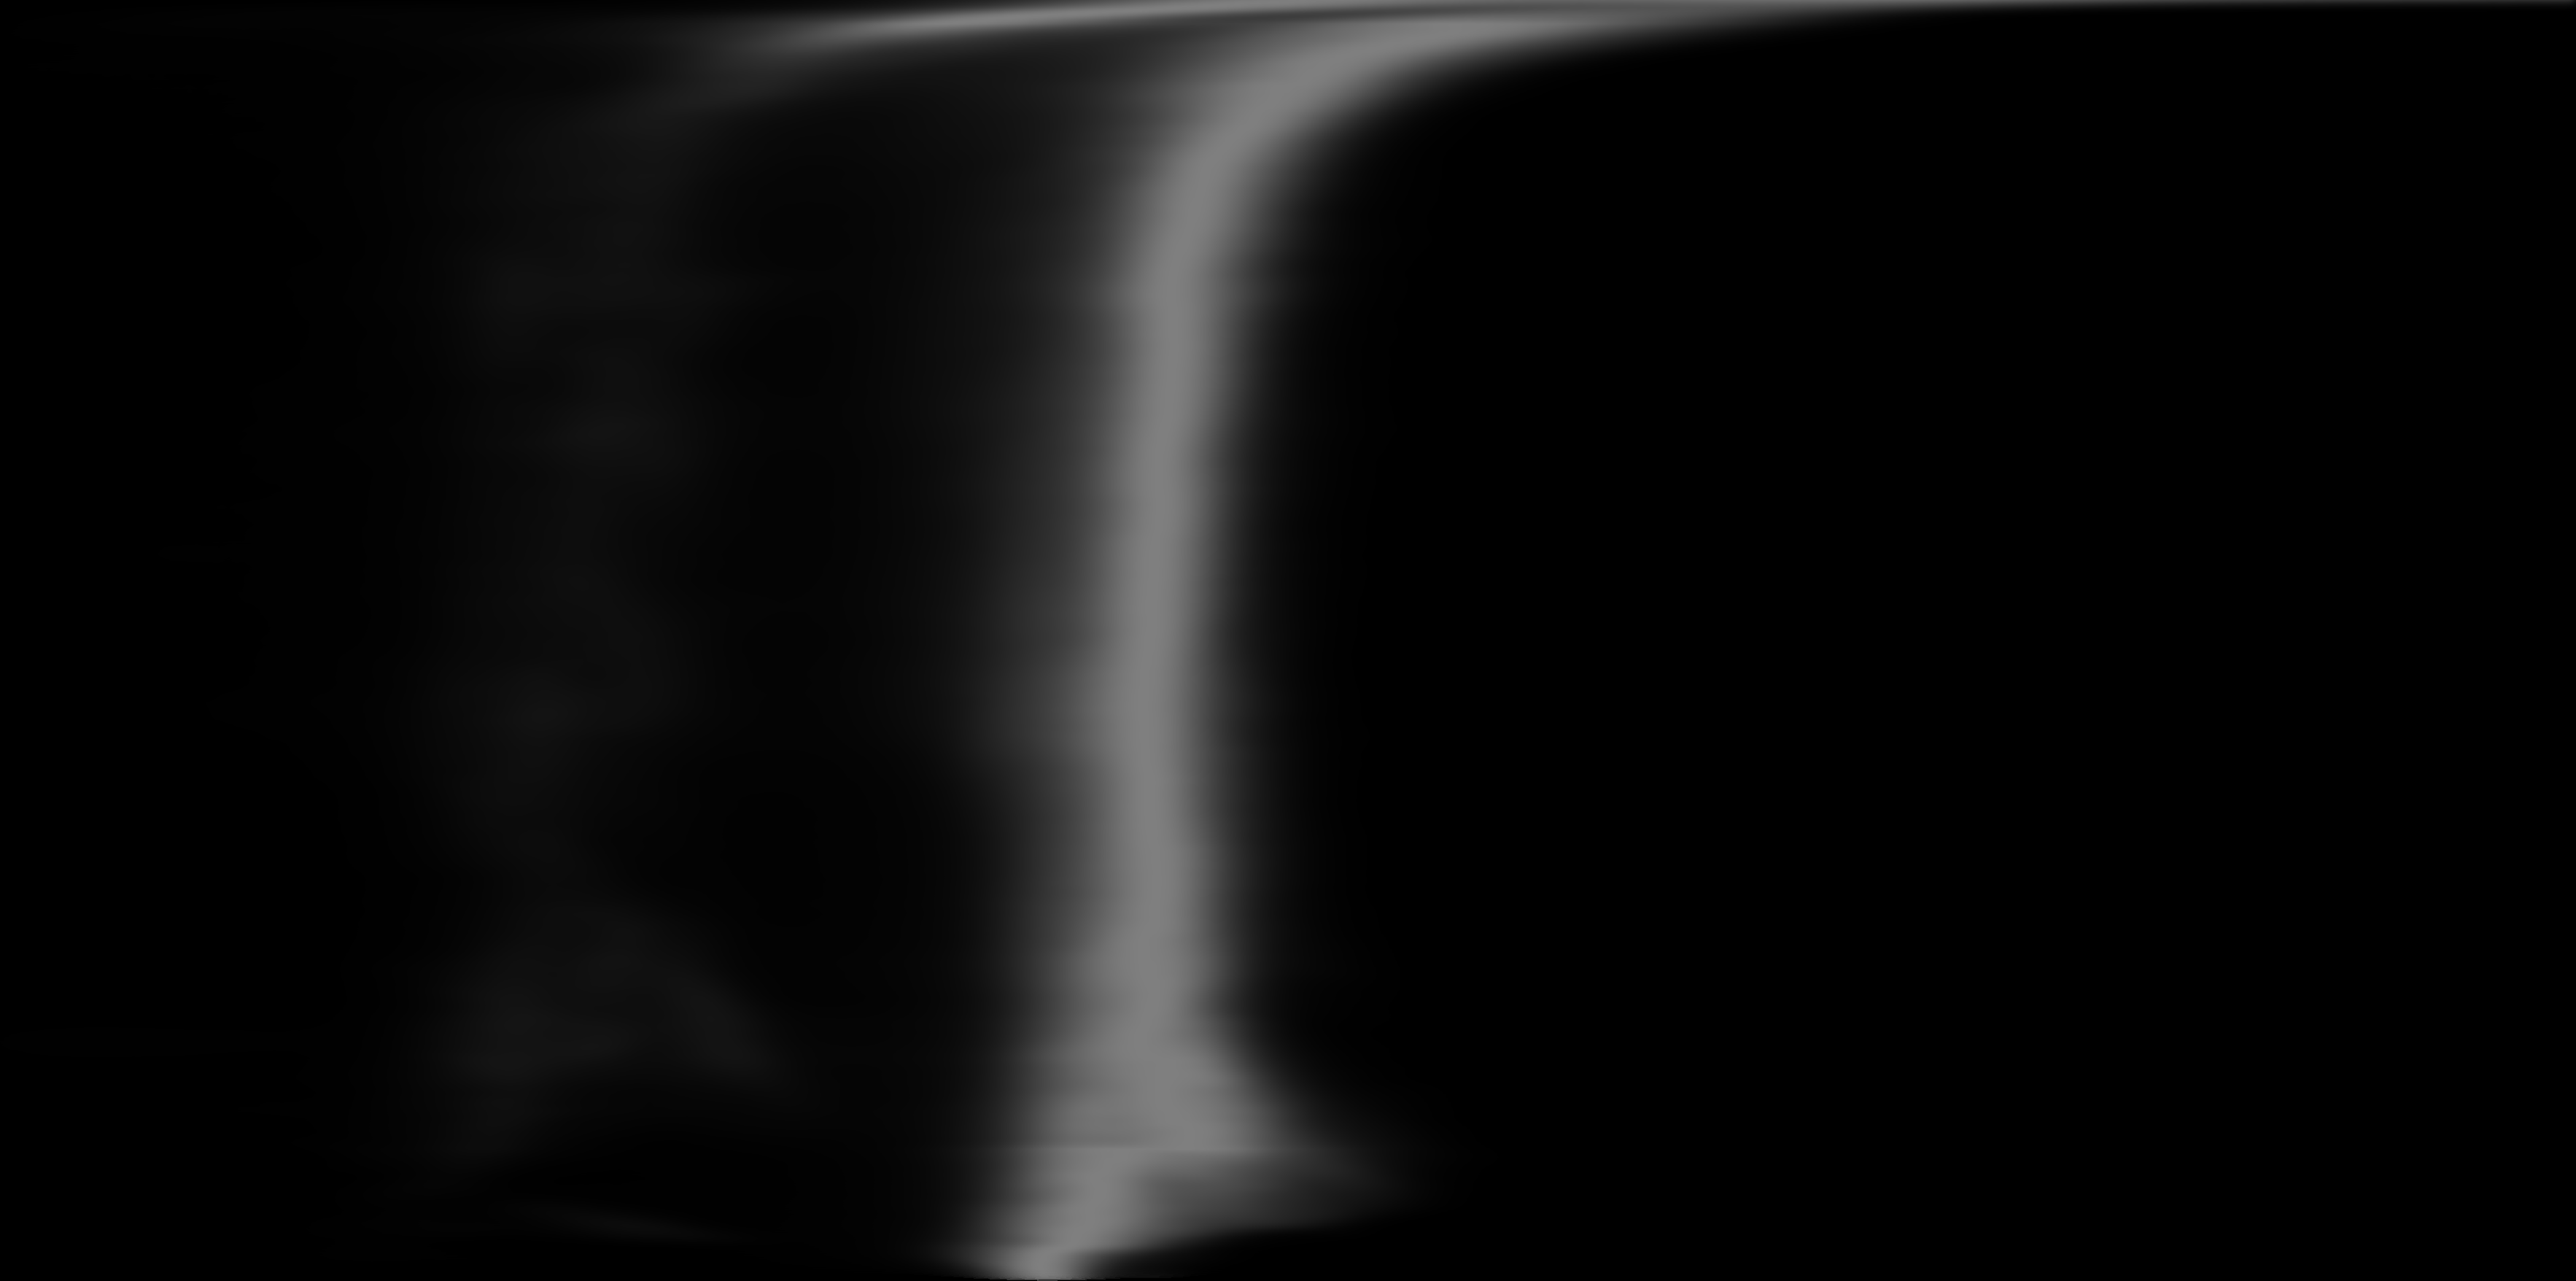
\includegraphics[width=\linewidth]{figures/fb-edt-bone_region3.png}
    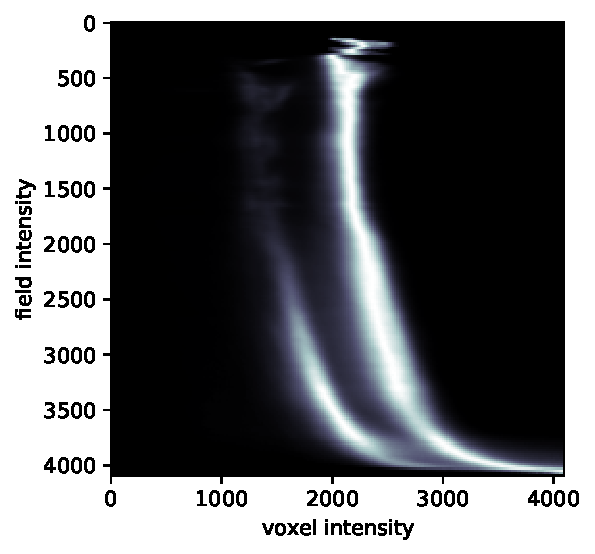
\includegraphics[width=\linewidth]{figures/fb-gauss+edt-bone_region3.pdf}
    \caption{2D field histogram. Note that there are two clearly seperated ridges, which make up the different materials.}
    \label{fig:field-hist}
\end{figure}

\vspace{\baselineskip}
\noindent\textbf{3. Isolate the materials} \\
The next step is to isolate the different materials spatially, which is done through the field histogram.
For our first attempt, we applied otsu's threshold to each each row in the 2D histogram. 
While this provided good results for two clearly defined distributions, it started to fail both because of lack of samples or because the histogram did not contain two distributions, which is an assumption of the otsu threshold. 
These two effects occurred in the edges (both closest and furthest), which would bleed into the later steps of the segmentation process. 

Our next solution was to rather than finding the threshold value in between the distributions, we started finding the distributions by finding the ridges of the 2D histogram. 
We do this by applying a series of image processing techniques, which~\Cref{alg:material} describes.
Each of the resultiong contours become their own material, which are then labeled as material 1 and 2 respectively for this particular sample. For samples that would contain more than two distributions, the same algorithm should apply, as long as the distributions does not overlap. 

\begin{algorithm}
    \caption{Material isolation.}
    \label{alg:material}
    \begin{algorithmic}
        \Function {Materials} {$h[f_{bins},v_{bins}],\sigma, peak_{min}, k_x, k_y, i_{dilate},$ \newline $i_{erode}, t$}
            \For {$row$ \textbf{in} $0{:}f_{bins}$}
                \State $r \gets gaussian\_smooth(h[row,:], \sigma)$
                \State $p \gets find\_peaks(r, peak_{min})$
                \State $ps[p] \gets 1$
            \EndFor
            \State $kernel = cross\_kernel(k_x, k_y)$
            \State $d \gets dilate(ps, i_{dilate}, kernel)$
            \State $e \gets erode(d, i_{erode}, kernel)$
            \State $cs \gets find\_contours(e)$
            \For {$i$ \textbf{in} $0{:}|cs|$}
                \If {$size(cs[i]) > t$}
                    \State $l \gets draw\_contour(l, cs[i], i+1)$
                \EndIf
            \EndFor
            \Return $l$
        \EndFunction
    \end{algorithmic}
\end{algorithm}

\begin{figure}
    %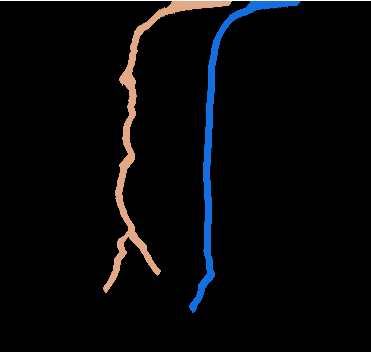
\includegraphics[width=0.5\linewidth]{figures/curves_edt.png}%
    %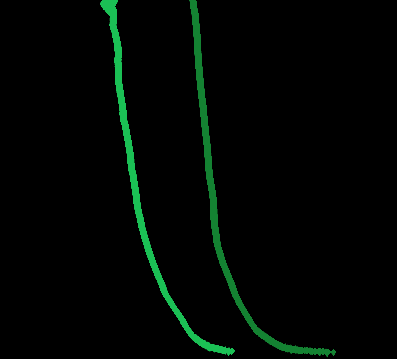
\includegraphics[width=0.5\linewidth]{figures/curves_diffusion.png}
    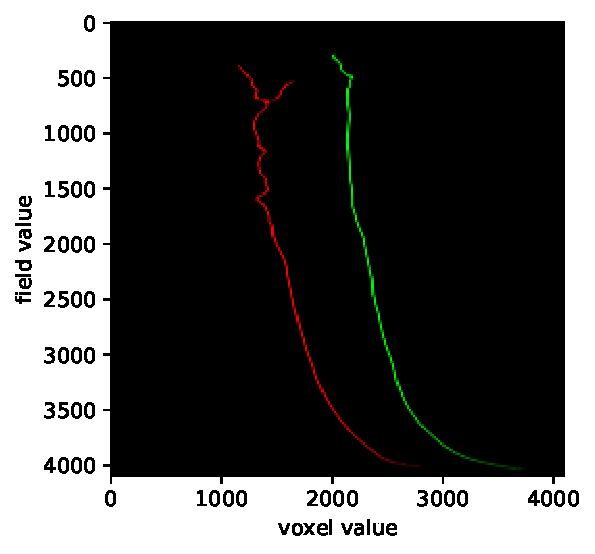
\includegraphics[width=\linewidth]{figures/ridges_gauss+edt-bone_region3.pdf}
    \carl{intermediate images of all of the steps?}
    \caption{Detected ridges from the combined field histogram.}
    \label{fig:curves}
\end{figure}

\vspace{\baselineskip}
\noindent\textbf{4. Compute models for material probability distributions} \\
Our goal is to obtain good conditional probability distributions $P(m|v,\xx)$
that model the likelihood of a voxel having material type $m$ as a function
both on its value $v$ and its position $\xx$ in space. For the probabilities
conditioned on the field values (distance or diffusion field), we model
the probability distributions $P(m|v,f(\xx))$ conditioned on
voxel- and field values. We want to make sure that these distribution
functions vary smoothly across space (or as a function of field values),
to ensure that we can identify the materials correctly across the entire
image: i.e., even though the frequency distributions look completely different
close to the titanium implant compared to the middle region or sample surface,
we can track the unbroken, smooth deformation to assign a global material
identity.

To this end, we first {\it model the frequency distributions} using the
2D histograms. Given that we are modeling materials $m=1,\ldots,M$,
we write the full 2D histogram as a sum of distributions
$g_m(\fval,v)$ modeling the described part, and an undescribed
residual $r(\xx,v)$.
\begin{equation}
  \label{eq:hist}
  H(\fval,v) = \sum_{m=1}^M g_m(\fval,v) + r(\fval,v)
\end{equation}
The residual is constrained to be non-negative, i.e., we must not explain
more voxels than the image contains.
The distribution functions can be chosen in any way that approximately
model the observed frequencies: we first used Gaussians with passable success,
but found that they dropped off too rapidly. We instead found excellent results
with the next-simplest model, leaving the exponential power free:
\begin{equation}
  \label{eq:dist-form}
  g_m(\fval,v) = a_m(\fval) e^{-b_m(\fval) |v-c_m(\fval)|^d_m(\fval)}
\end{equation}
where for each field value $\fval$
$a(\fval)$ is the distribution height at the center $v=c(\fval)$,
$b(\fval)$ is the exponential falloff rate, and $d(\fval)$ is
the exponential power ($d=2$ yields a Gaussian, $d=1$ a simple exponential).
In practice we found $1.5\le d \le 2$ to best match the actual frequency
distribution decay rates.

Using the ridges found in the previous step, we generate good starting
guesses and constraints for the distribution parameters
$a,b,c,d$:
For each field-value $\fval$ (corresponding to a row in the 2D histogram),
we initialize the starting approximation as:
\begin{equation}
  \label{eq:starting-guesses}
  \begin{split}
    c_m(\fval) &= \mathop{\mathtt{argmax}}_{v \text{ with }\lab[\fval,v] = m} H(\fval,v)    \\
    a_m(\fval) &= H(\fval,c_m(\fval))\\
    b_m(\fval) &= 3/\mathrm{width}_m(\fval)^2 \\
    d_m(\fval) &= 2
  \end{split}
\end{equation}
where we use half the distance to the center of ridge $m+1$ as the width
$\mathrm{width_m}(\fval)$, using the relation that $b = 3/w^d$ yields
a $5\%$ cutoff at $w$ when $1\le d \le 2$. This approximation
already yields a good approximation. Thus, the subsequent
optimization using the constrained quasi-Newton optimization method L-BFGS-B\cite{BFGS}
converges rapidly to an excellent fit. Each 1D histogram row is first optimized
independently in parallel: The resulting numerical functions
$a_m(\fval),\ldots,d_m(\fval)$ are then converted into piecewise cubic
functions using a least squares-based algorithm that ensures continuity
and differentiability across the piecewise segments. This lets us interpolate across
outliers due to noise, but equally important:
extrapolate our models smoothly into the regions very close to the implant, where
we don't have enough voxels to produce good statistics.

We finally obtain the {\it conditional probabilities} from the material frequency distribution
models $g_m$ as:
\begin{equation}
  \label{eq:Pm}
  P(m|v,f(\xx)) = \frac{g_m(v,f(\xx))}{H(v,f(\xx))}
\end{equation}
(well-defined where $H(v,\fval) > 0$, zero outside this region as $0\le g_m \le H$).



%%% Local Variables:
%%% mode: latex
%%% TeX-master: "main"
%%% End:


\vspace{\baselineskip}
\noindent\textbf{5. Perform segmentation}

The final step of the segmentation process is to utilize the probabilities for segmentation.
This process is fairly straightforward, as each voxel is looked up in the probability distribution, which carries the same shape as the field histogram.

\begin{algorithm}
    \caption{Final segmentation from the probability distributions.}
    \label{alg:segment}
    \begin{algorithmic}
        \Function {Segment} {$voxels[n_z,n_y,n_x], p[f_{bins},v_{bins}],$ \newline $v_{bins}, v_{min}, v_{max}, f_{bins}, f_{min}, f_{max}$}
            \For {$z,y,x$ \textbf{in} $0{:}n_z,0{:}n_y,0{:}n_x$}
                \State $v \gets voxels[z,y,x]$
                \If {$v_{min} \leq v \leq v_{max}$}
                    \State $f \gets voxels[z,y,x]$
                    \If {$f_{min} \leq f \leq f_{max}$}
                        \State $v_i \gets (v_{bins} - 1) - \frac{v - v_{min}}{v_{max} - v_{min}}$
                        \State $f_i \gets (f_{bins} - 1) - \frac{f - f_{min}}{f_{max} - f_{min}}$
                        \State $result[z,y,x] \gets p[f_i, v_i]$
                    \EndIf
                \EndIf
            \EndFor
            \Return $result$
        \EndFunction
    \end{algorithmic}
\end{algorithm}

\subsection{Results of the field segmentation}

\subsubsection{Sub-classification of soft tissue}

With a separation of soft tissue and bone in hand, we 
map out the blood vessel network using connected components analysis. 
The osteocytes are selected by volume and shape: for every connected
component in the feasible volume range, its principal axis and best
ellipsoid is computed and checked against the potential osteocyte shape.

\subsection{Visualizing bone-implant contact and blood-implant contact}

Using a Euclidean Distance Transform (EDT) from the implant, restricted to the
bone region, we can simply mask the voxels that are within a thin shell
of distances, $d_{min} < d(x,y,z) \le d_{max}$. We choose $d_{min} = 0$ and
$d_{max} = 10\mu m$.
We then simply sum over the masked voxels of each tissue type to obtain
and divide by the total to obtain the tissue-to-implant contact per area.
However, this only yields a single number, and it is difficult to verify
its fidelity.

\subsubsection{Histology-comparison}

\begin{figure}
  \centering
  \begin{tabular}{c}
    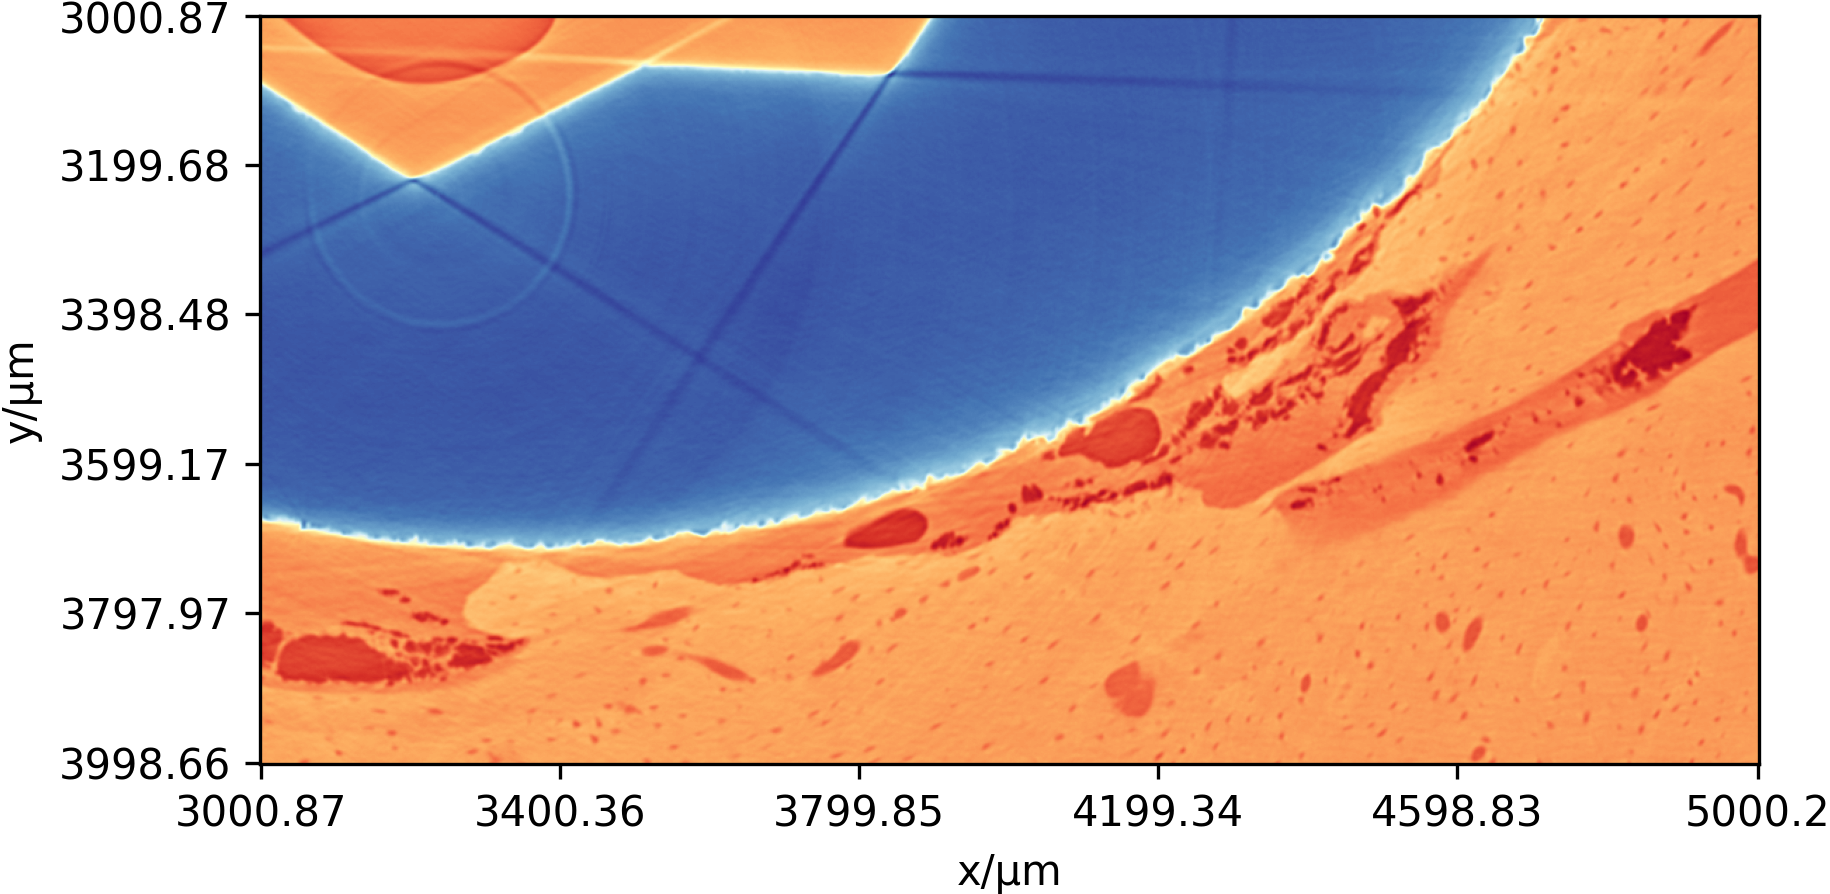
\includegraphics[width=\linewidth]{figures/770c_pag-bic-xy-1x} \\
    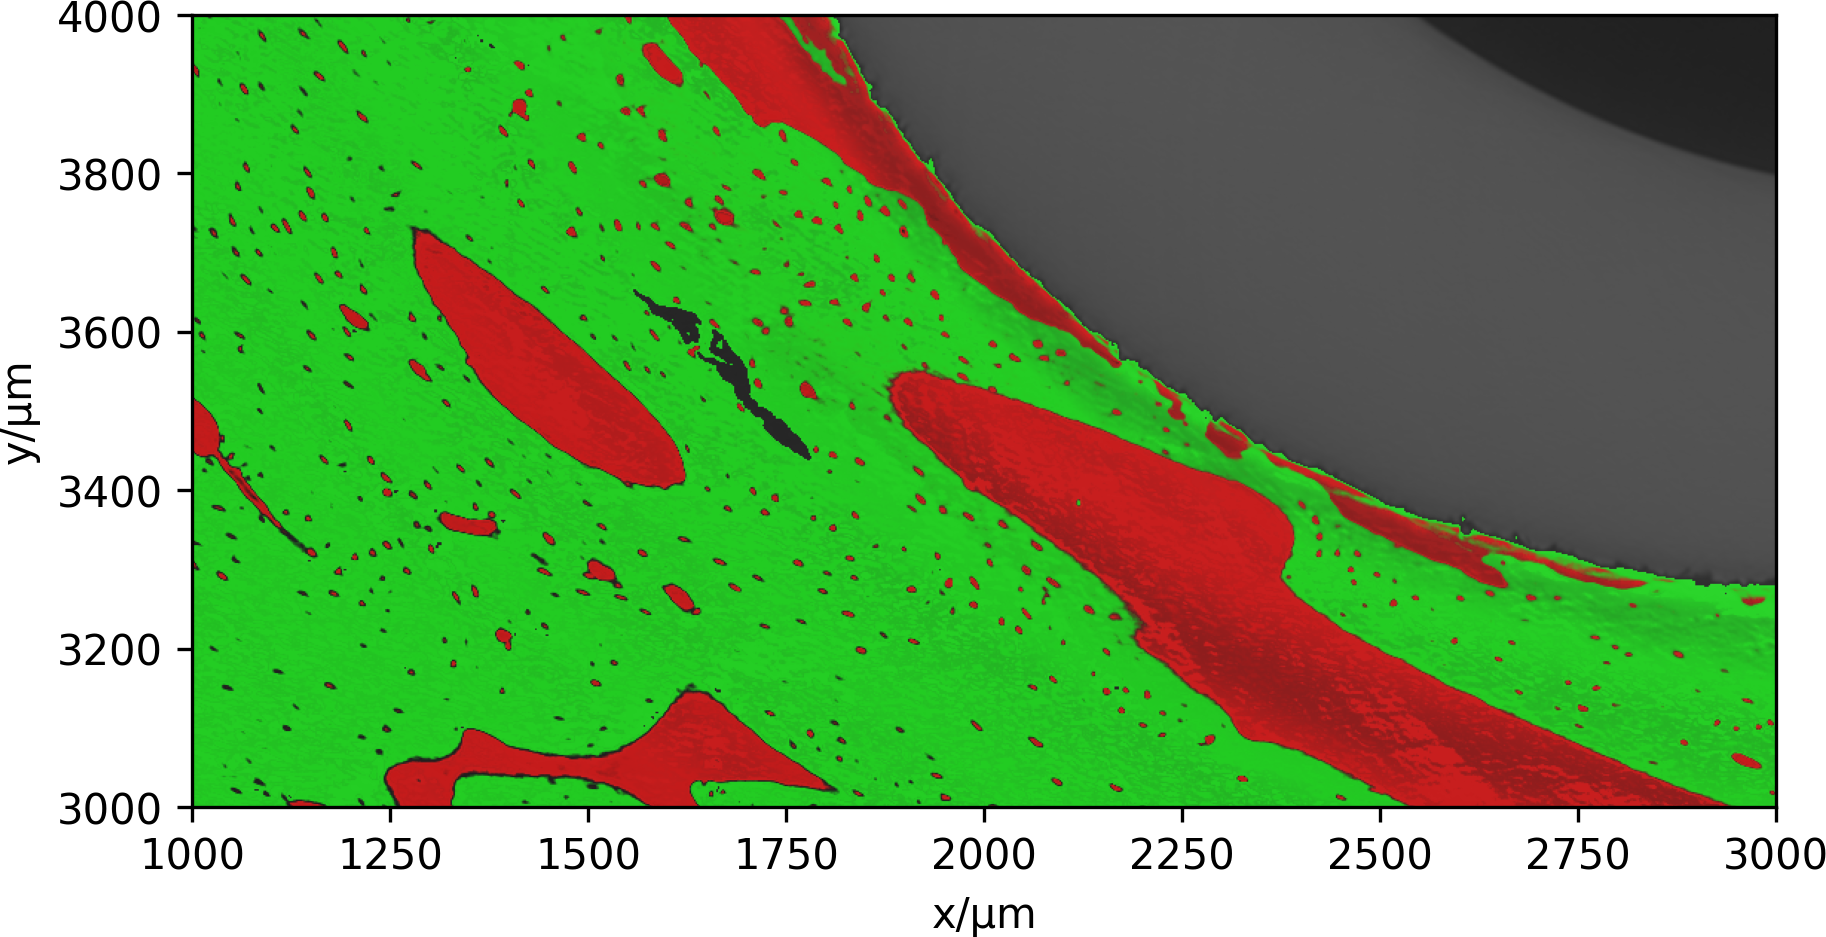
\includegraphics[width=\linewidth]{figures/770c_pag-bic-P01-xy-1x}
  \end{tabular}
  \caption{TBW}
  \label{fig:histology-comparison1}
\end{figure}

\begin{figure}
  \centering
  \begin{tabular}{c}
    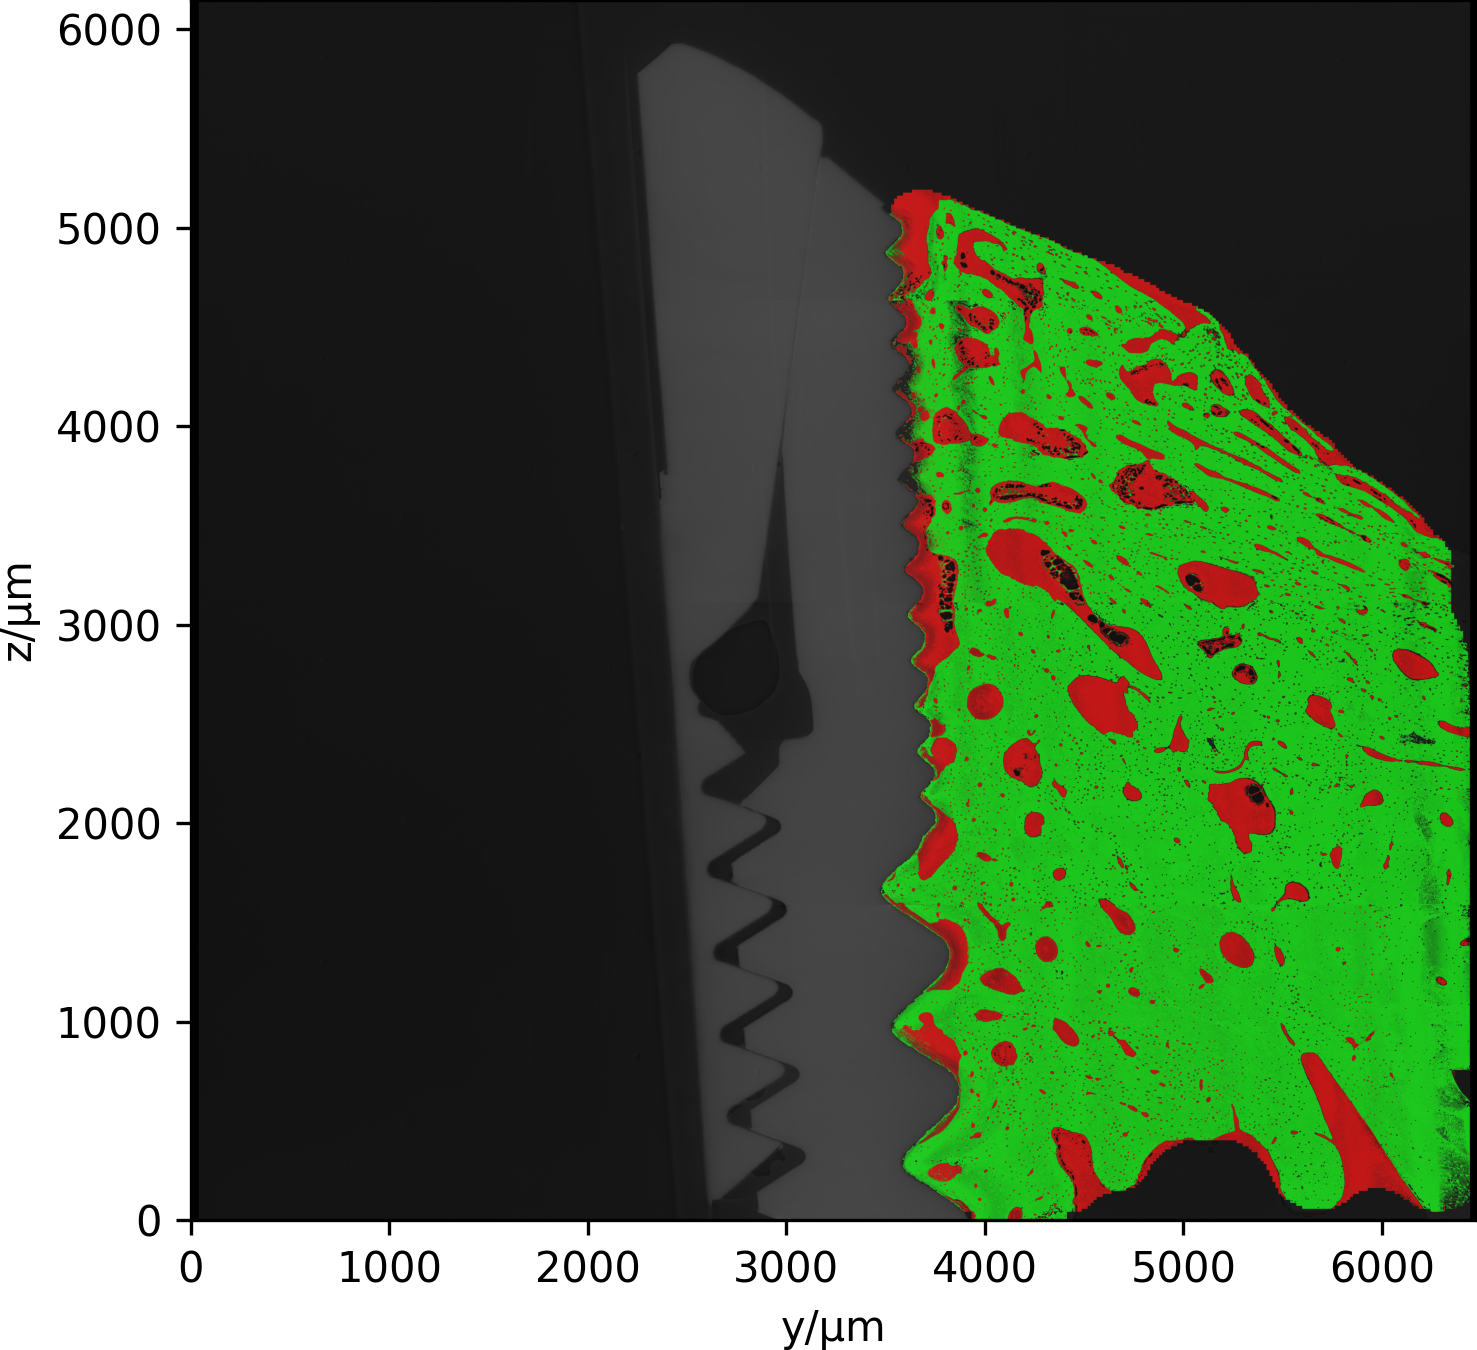
\includegraphics[width=\linewidth]{figures/770c_pag-full-P01-yz-1x} \\
    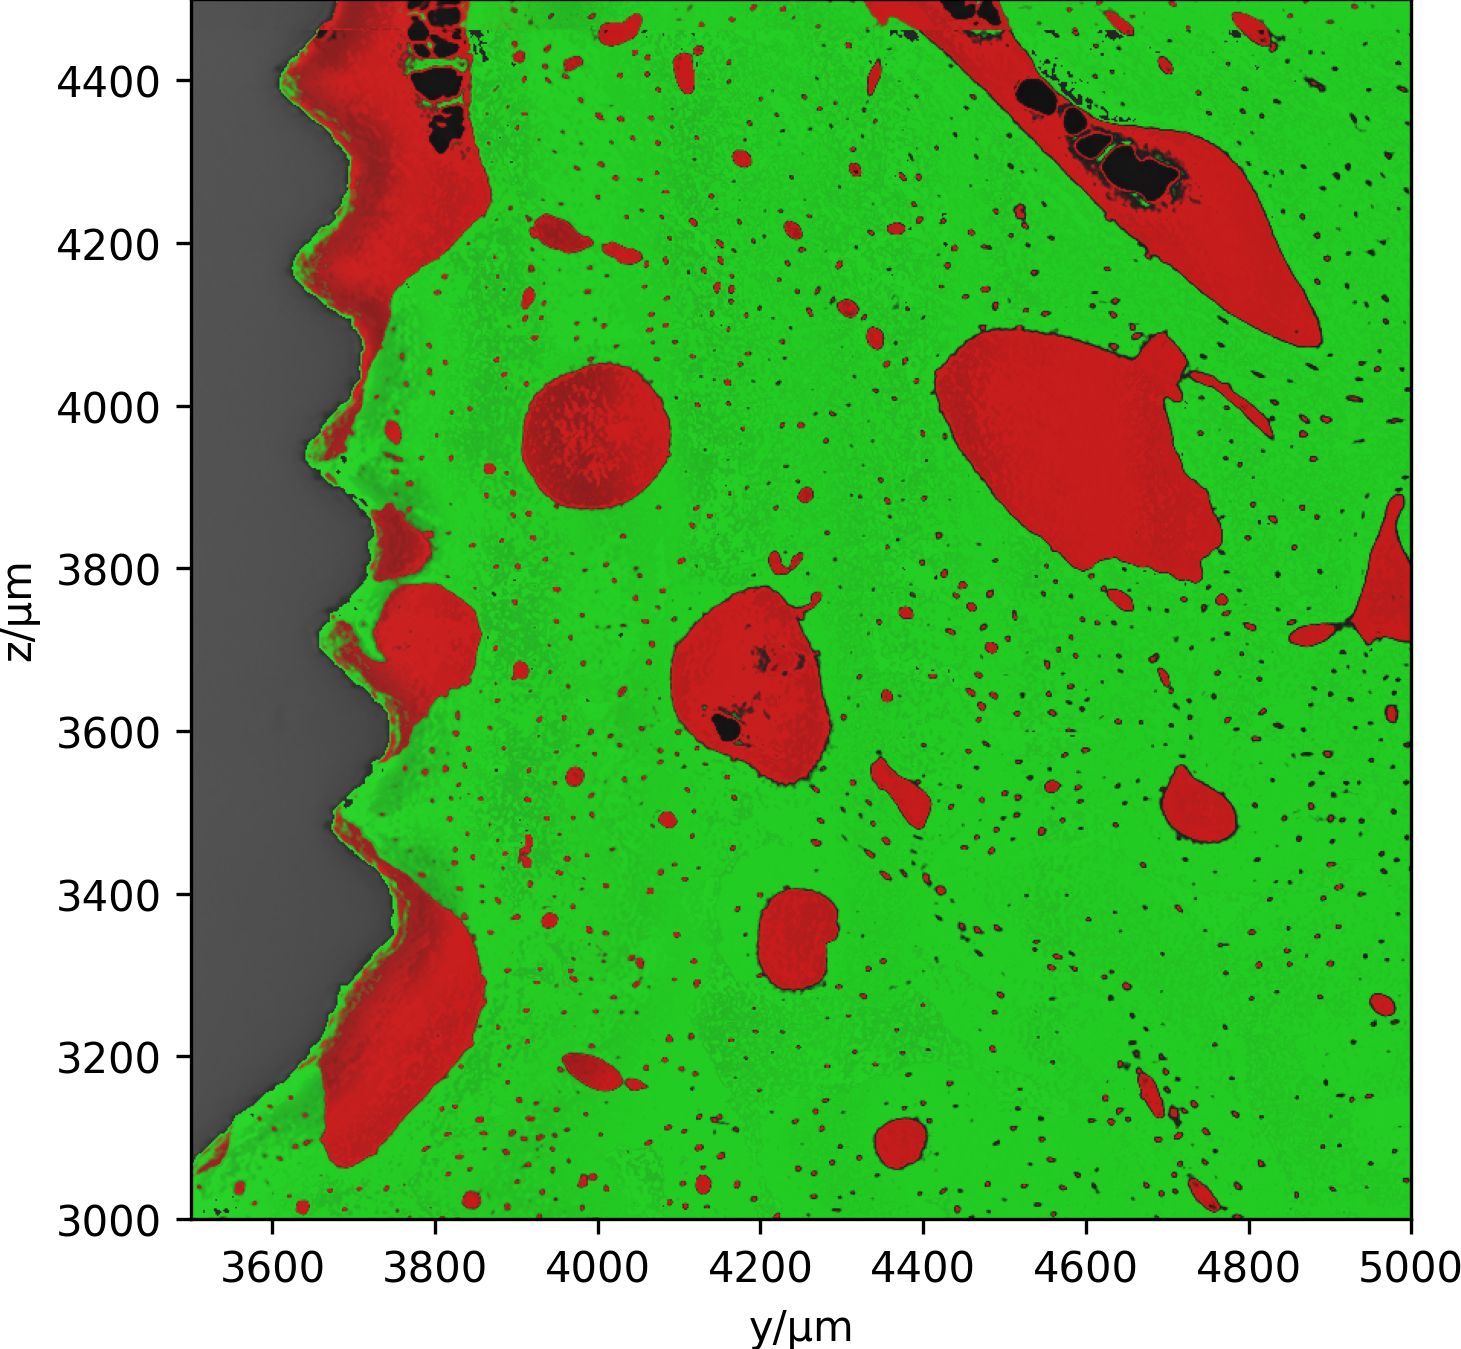
\includegraphics[width=\linewidth]{figures/770c_pag-bic-P01-yz-1x}
  \end{tabular}
  \caption{TBW}
  \label{fig:histology-comparison2}
\end{figure}

\subsubsection{Cylindrical projection of implant contact-surface}

In this subsection, we show how to map the tissue-to-implant contact
surface for visual inspection. The challenge is that the equidistant
region forms a curved surface that cannot simply be flattened. Instead,
we project the voxels onto a cylinder, as shown on Figure \ref{fig:cylinder1}.

\begin{figure}
  \centering
  \begin{tabular}{cc}
    (a) & \begin{tabular}{c}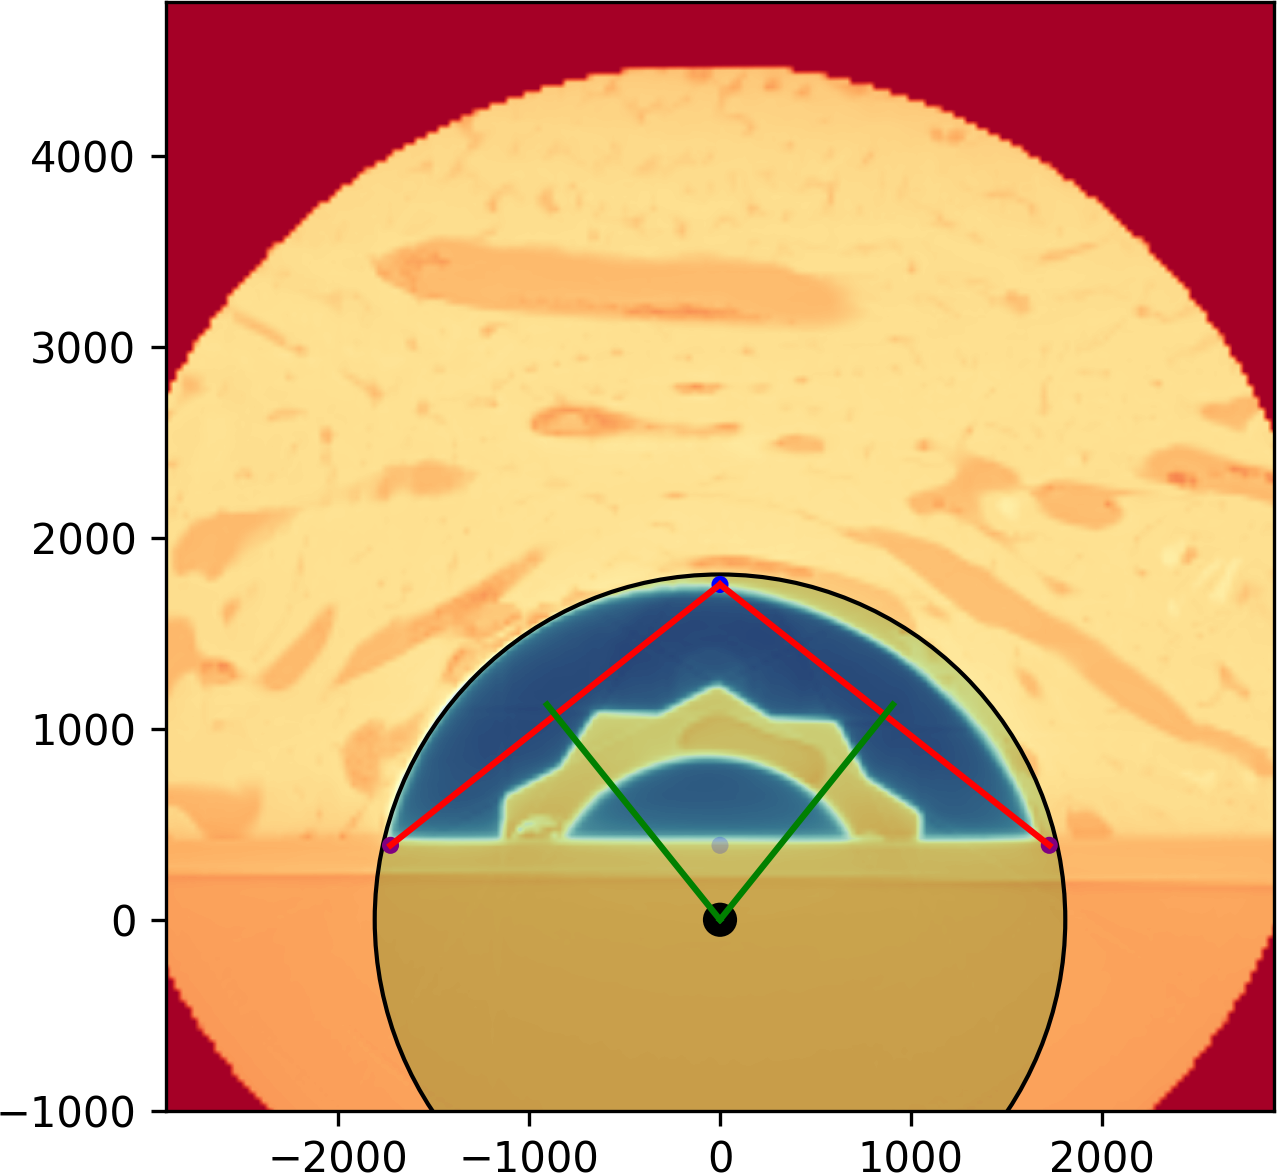
\includegraphics[width=.8\linewidth]{figures/implant-FoR_prime-circle}\end{tabular} \\
    (b) & \begin{tabular}{c}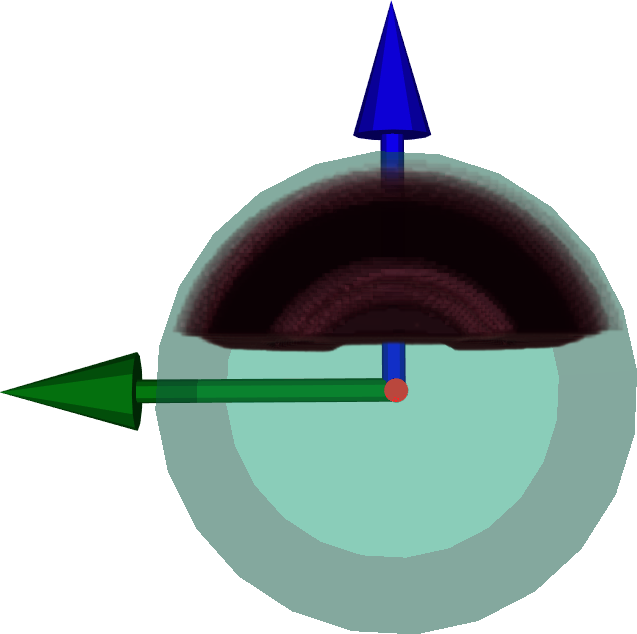
\includegraphics[width=0.4\linewidth]{figures/implant-FoR_cylinder-y}%
  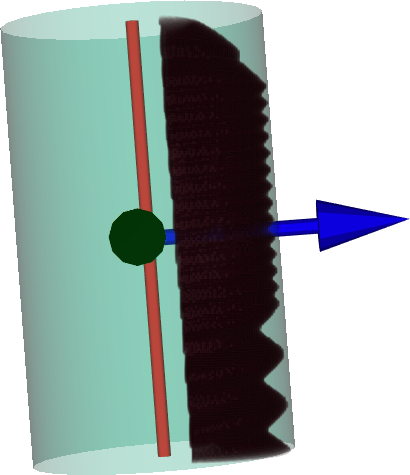
\includegraphics[width=0.5\linewidth]{figures/implant-FoR_cylinder-z2}\end{tabular}
  \end{tabular}
  \caption{
    (a) The implant is divided into 100 segments along its principal axis,
    and for each segment, the circumscribed circle is computed. 
    (b) The best overall cylindrical fit for the implant is computed using
    least squares. The implant contact are projected onto this cylinder,
    and can now be shown in a flat plot.}
  \label{fig:cylinder1}
\end{figure}





%%% Local Variables:
%%% mode: latex
%%% TeX-master: "main"
%%% End:
